%%%%%%%%%%%%%%%%%%%%%%%%%%%%%%%%%%%%%%%%%
% Focus Beamer Presentation
% LaTeX Template
% Version 1.0 (8/8/18)
%
% This template has been downloaded from:
% http://www.LaTeXTemplates.com
%
% Original author:
% Pasquale Africa (https://github.com/elauksap/focus-beamertheme) with modifications by 
% Vel (vel@LaTeXTemplates.com)
%
% Template license:
% GNU GPL v3.0 License
%
% Important note:
% The bibliography/references need to be compiled with bibtex.
%
%%%%%%%%%%%%%%%%%%%%%%%%%%%%%%%%%%%%%%%%%

%----------------------------------------------------------------------------------------
%	PACKAGES AND OTHER DOCUMENT CONFIGURATIONS
%----------------------------------------------------------------------------------------

\documentclass[aspectratio=1610, professionalfonts, 10pt]{beamer}
\usepackage{polyglossia}
\setmainlanguage{german}
\usepackage[
  locale=DE,                 % deutsche Einstellungen
  separate-uncertainty=true, % immer Fehler mit \pm
  per-mode=reciprocal,       % ^-1 für inverse Einheiten
  % alternativ:
  % per-mode=reciprocal, % m s^{-1}
  % decimal-marker=., % . statt , f�r Dezimalzahlen
]{siunitx}

\usepackage[
  version=4,
  math-greek=default, % ┐ mit unicode-math zusammenarbeiten
  text-greek=default, % ┘
]{mhchem}

\usetheme{focus} % Use the Focus theme supplied with the template
% Add option [numbering=none] to disable the footer progress bar
% Add option [numbering=fullbar] to show the footer progress bar as always full with a slide count

% Uncomment to enable the ice-blue theme
%\definecolor{main}{RGB}{92, 138, 168}
%\definecolor{background}{RGB}{240, 247, 255}



%------------------------------------------------

\usepackage{booktabs} % Required for better table rules

\usepackage{url}

\usepackage{chronology}



%----------------------------------------------------------------------------------------
%	 TITLE SLIDE
%----------------------------------------------------------------------------------------

\title{Die W-/Z-Boson Entdeckung}

%\subtitle{Subtitle}

\author{Jean-Marco Alameddine}

%\titlegraphic{
\includegraphics[scale=1.25]{Images/focuslogo.pdf}} % Optional title page image, comment this line to remove it

\institute{TU Dortmund \\ Fakultät Physik}

\date{07 12 2018}

%------------------------------------------------

\begin{document}

%------------------------------------------------

\begin{frame}
	\maketitle % Automatically created using the information in the commands above
\end{frame}

\section{Die Theorie der schwachen Wechselwirkung}

\begin{frame}{Fermis Theorie des $\beta$-Zerfalls}
			\begin{itemize}
				\setlength\itemsep{0.5em}
				\item \textbf{1933} beschreibt Fermi den $\beta$-Zerfalls über die Fermi-Wechselwirkung
				\item Theorie beschreibt eine Vier-Fermionen-Wechselwirkung ohne Austauschteilchen
				\item [$\rightarrow$] Wechselwirkung als Produkt zweier Ströme
				\item [$\rightarrow$] Kopplungsstärke beschrieben durch Fermikonstante $G_\text{F}$
			\end{itemize}

			\begin{figure}
	  			\centering
				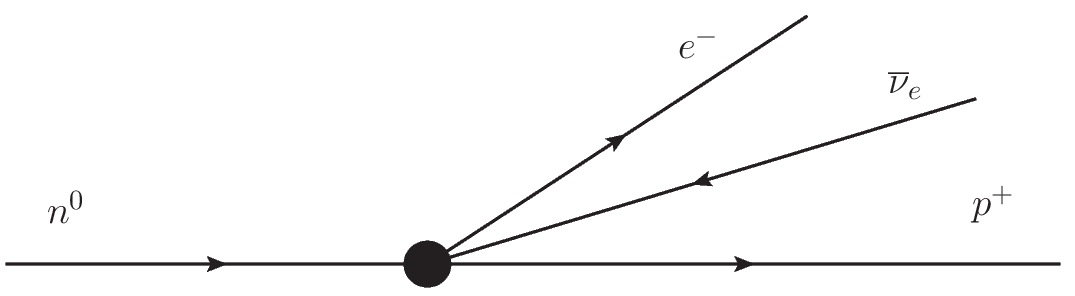
\includegraphics[width=0.9\linewidth]{Images/fourFermi_BetaDecay.png}
	  			\caption{Beschreibung des $\beta$-Zerfalls nach Fermi \cite{fermi_four}}
	  			\label{fig:fermi}
			\end{figure}
\end{frame}

\begin{frame}{Die Fermi-Wechselwirkung als effektive Theorie}
	\begin{figure}
	  	\centering
		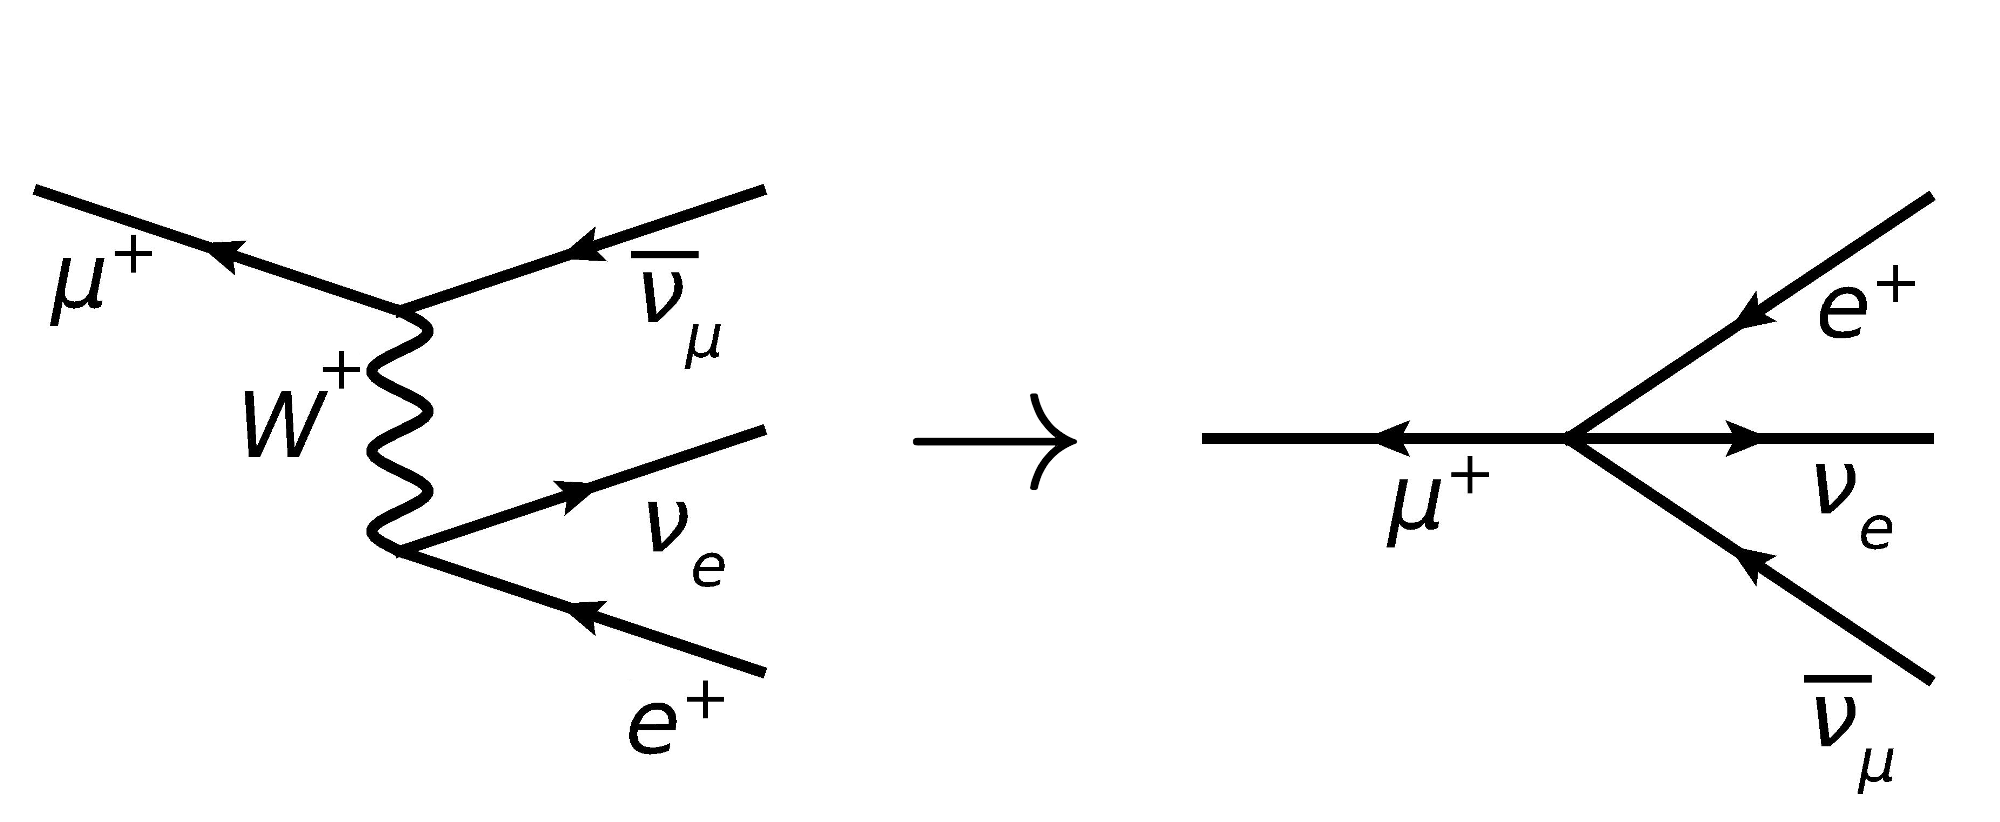
\includegraphics[width=0.8\linewidth]{Images/muon_decay.png}
	  	\label{fig:fermi_2}
	\end{figure}	
		\vspace*{-10px}
	\begin{columns}
		\column{0.45\textwidth}
				{\Large
				\begin{align*}
					\frac{-i \left( g_{\mu\nu} - \frac{q_\mu q_\nu}{M^2} \right)}{q^2 - M^2}
				\end{align*}
				}%
		\column{0.1\textwidth}
				{\LARGE
				\begin{align*}
					\underbrace{\rightarrow}_{q^2 \ll M^2}
				\end{align*}
				}%
		\column{0.45\textwidth}
				{\Large
				\begin{align*}
					\frac{i g_{\mu\nu}}{M^2}
				\end{align*}
				}%
	\end{columns}
	\vspace*{15px}
	\cite{Gorringe:2015cma} (bearbeitet), \cite{Griffiths:111880}
\end{frame}

\begin{frame}{Die Fermi-Wechselwirkung als effektive Theorie}
	\begin{columns}
		\column{0.6\textwidth}
			\begin{itemize}
				\setlength\itemsep{0.5em}
				\item Fermi-Wechselwirkung stellt für kleine Energien (bis heute) eine sehr gute Näherung dar (da schwache Wechselwirkung mit geringer Reichweite)
				\item Verallgemeinerung: Anwendung der Theorie auf viele weitere Reaktionen (z.B. $\mu$-Zerfall) liefert hervorragende Ergebnisse
				\item [$\rightarrow$] Erweiterung der Theorie, um neue Phänomene wie die Paritätsverletzung beschreiben zu können (V-A-Struktur)
			\end{itemize}
		\column{0.4\textwidth}
			\begin{figure}
	  			\centering
				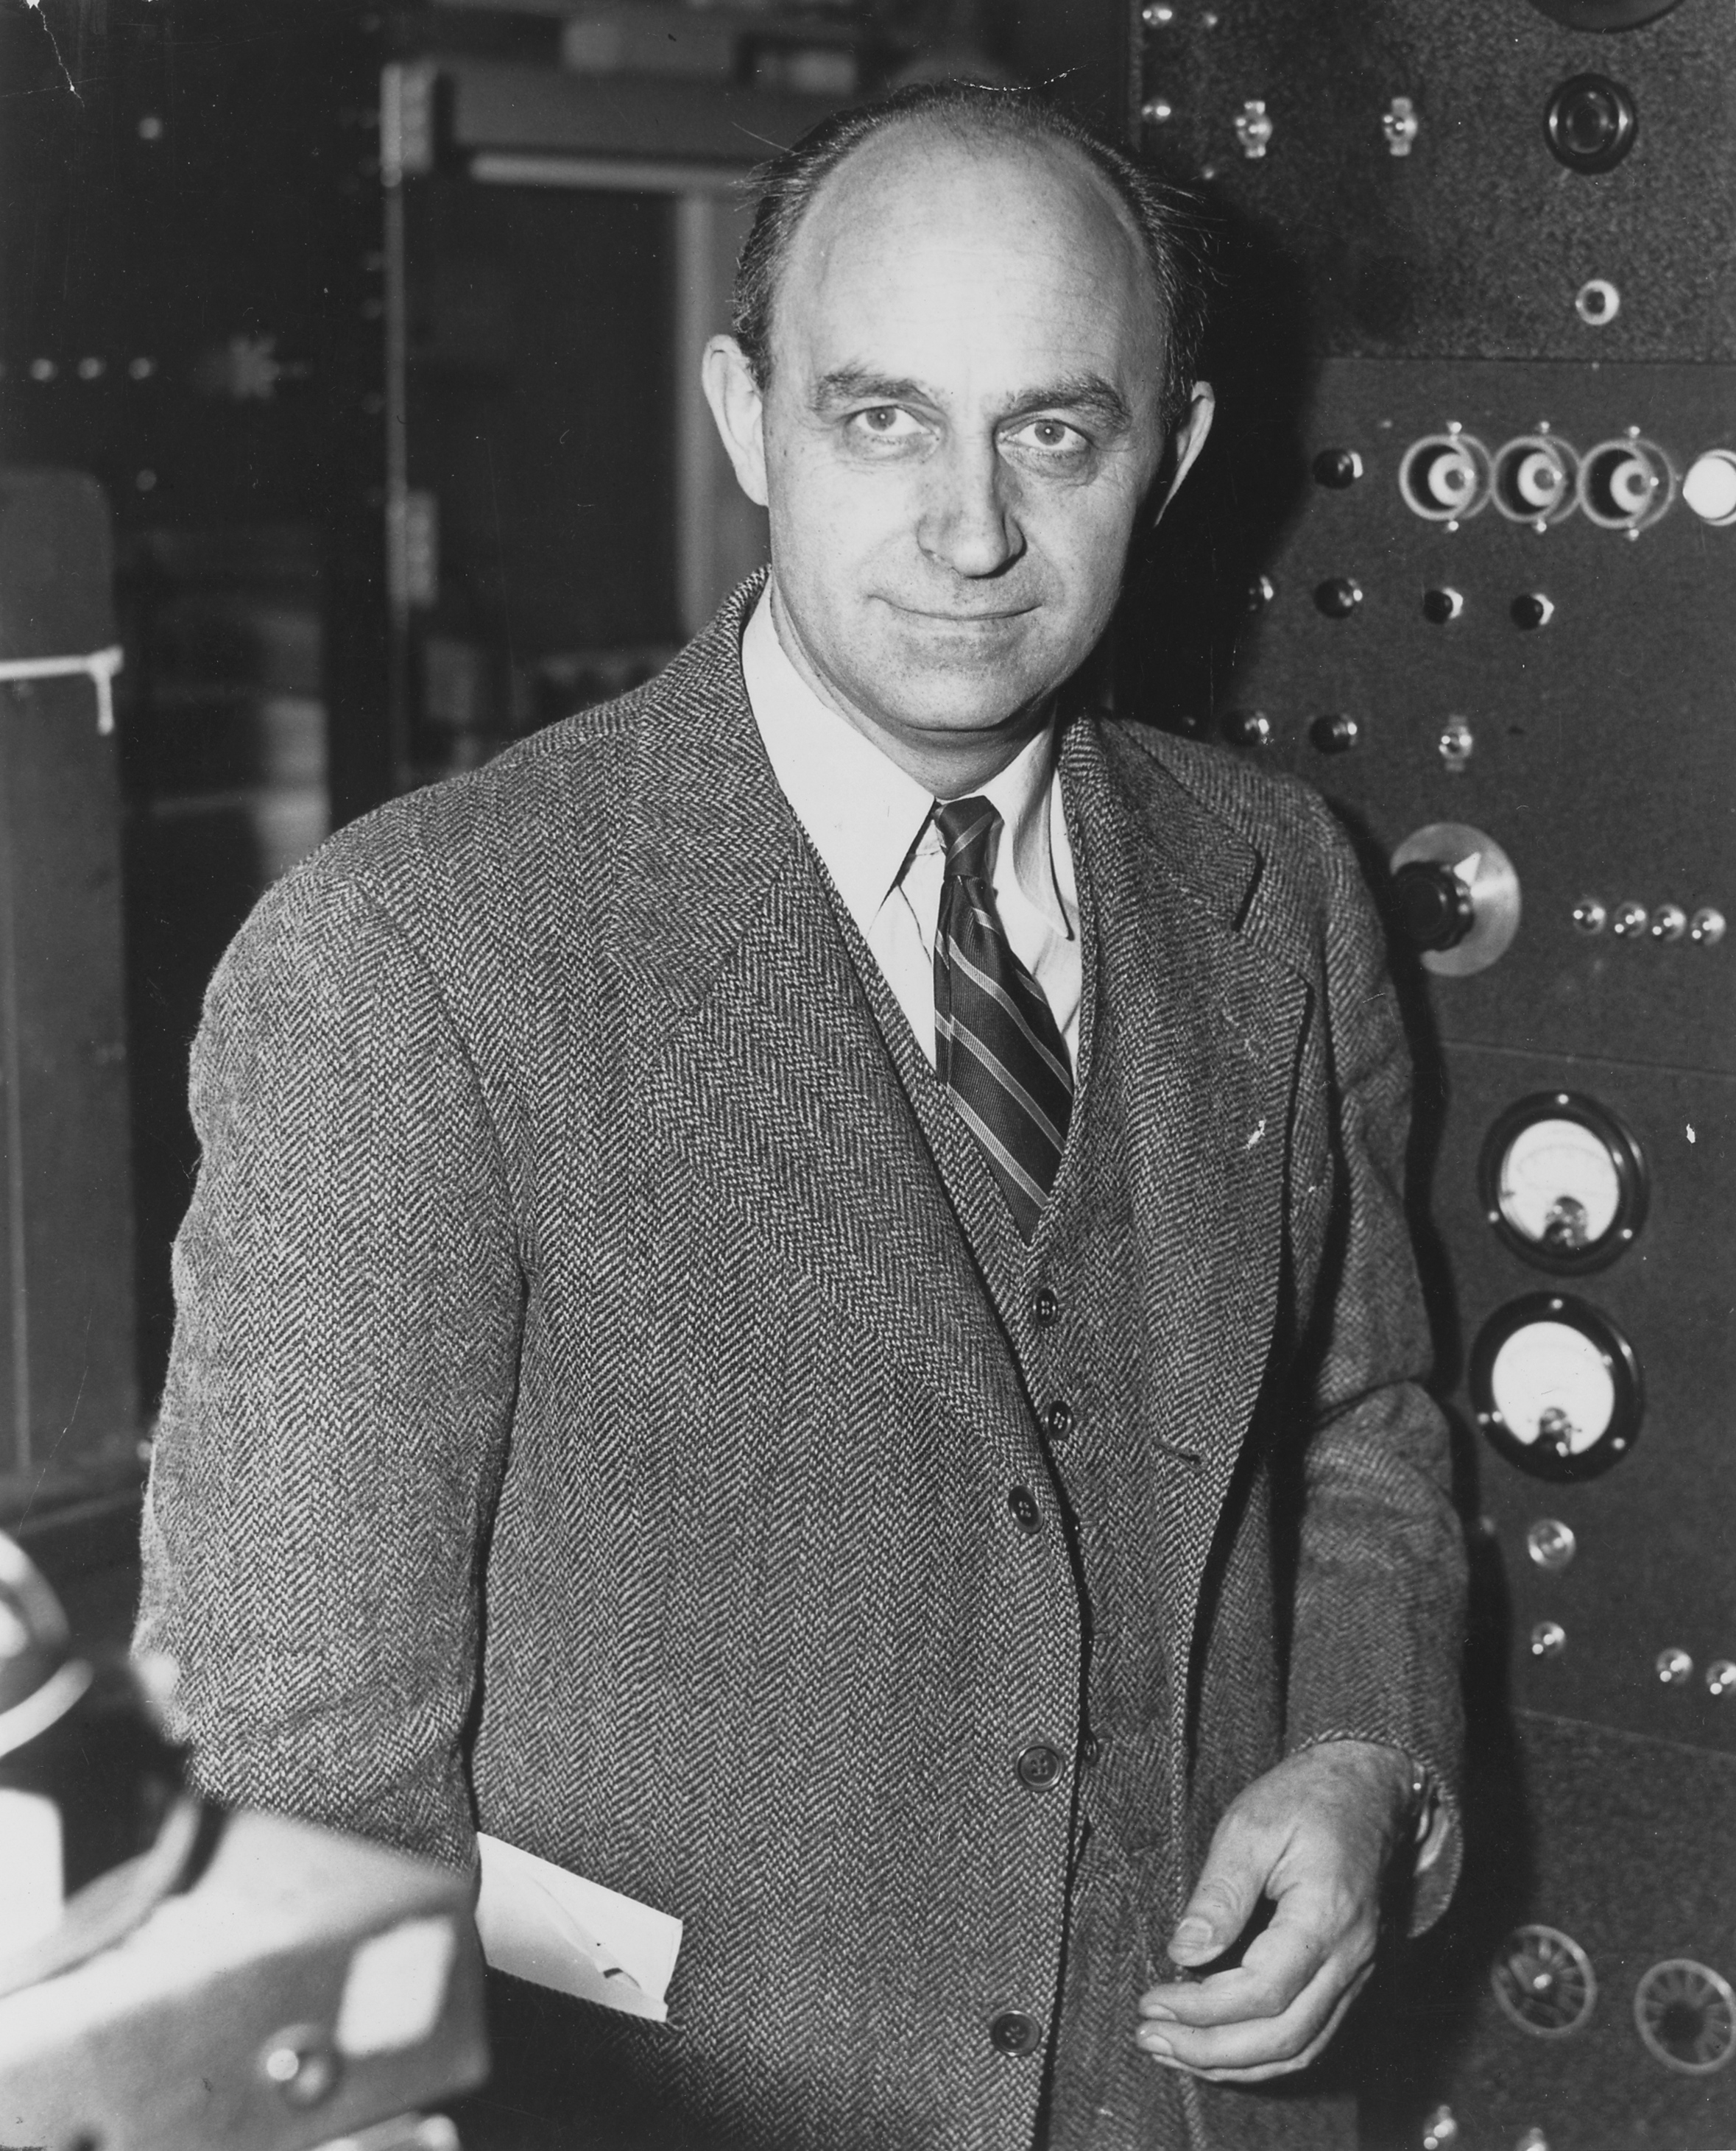
\includegraphics[width=\linewidth]{Images/Enrico_Fermi_1943-49.jpg}
	  			\caption{Enrico Fermi \cite{wiki:fermi}}
	  			\label{fig:fermi}
			\end{figure}
	\end{columns}
\end{frame}


\begin{frame}{Die Fermi-Wechselwirkung als effektive Theorie}
	\begin{columns}
		\column{0.6\textwidth}
			\begin{itemize}
				\setlength\itemsep{0.5em}
				\item Theorie der Fermi-Wechselwirkung nicht renormierbar
				\item [$\rightarrow$] Divergenzen bei höheren Energien bzw. höheren Ordnungen in $G_\text{F}$
			\end{itemize}
				\vspace*{10px}
			\begin{itemize}
				\item Ab $E \approx \SI{300}{\giga\electronvolt}$: Verletzung des "Unitarity limit"
				\item [$\rightarrow$] $\sigma \propto G_\text{F}^2 E^2$
				\item [$\rightarrow$] Bedingung an totalen Wirkungsquerschnitt, welche aus der Unitarität stammt, wird verletzt (unphysikalisch) \cite{perkins_2000}
			\end{itemize}
			\vspace*{10px}
			\begin{itemize}
				\item Mit höheren Beschleunigerenergien können Abweichungen von der Theorie gemessen werden
			\end{itemize}
		\column{0.4\textwidth}
			\begin{figure}
	  			\centering
				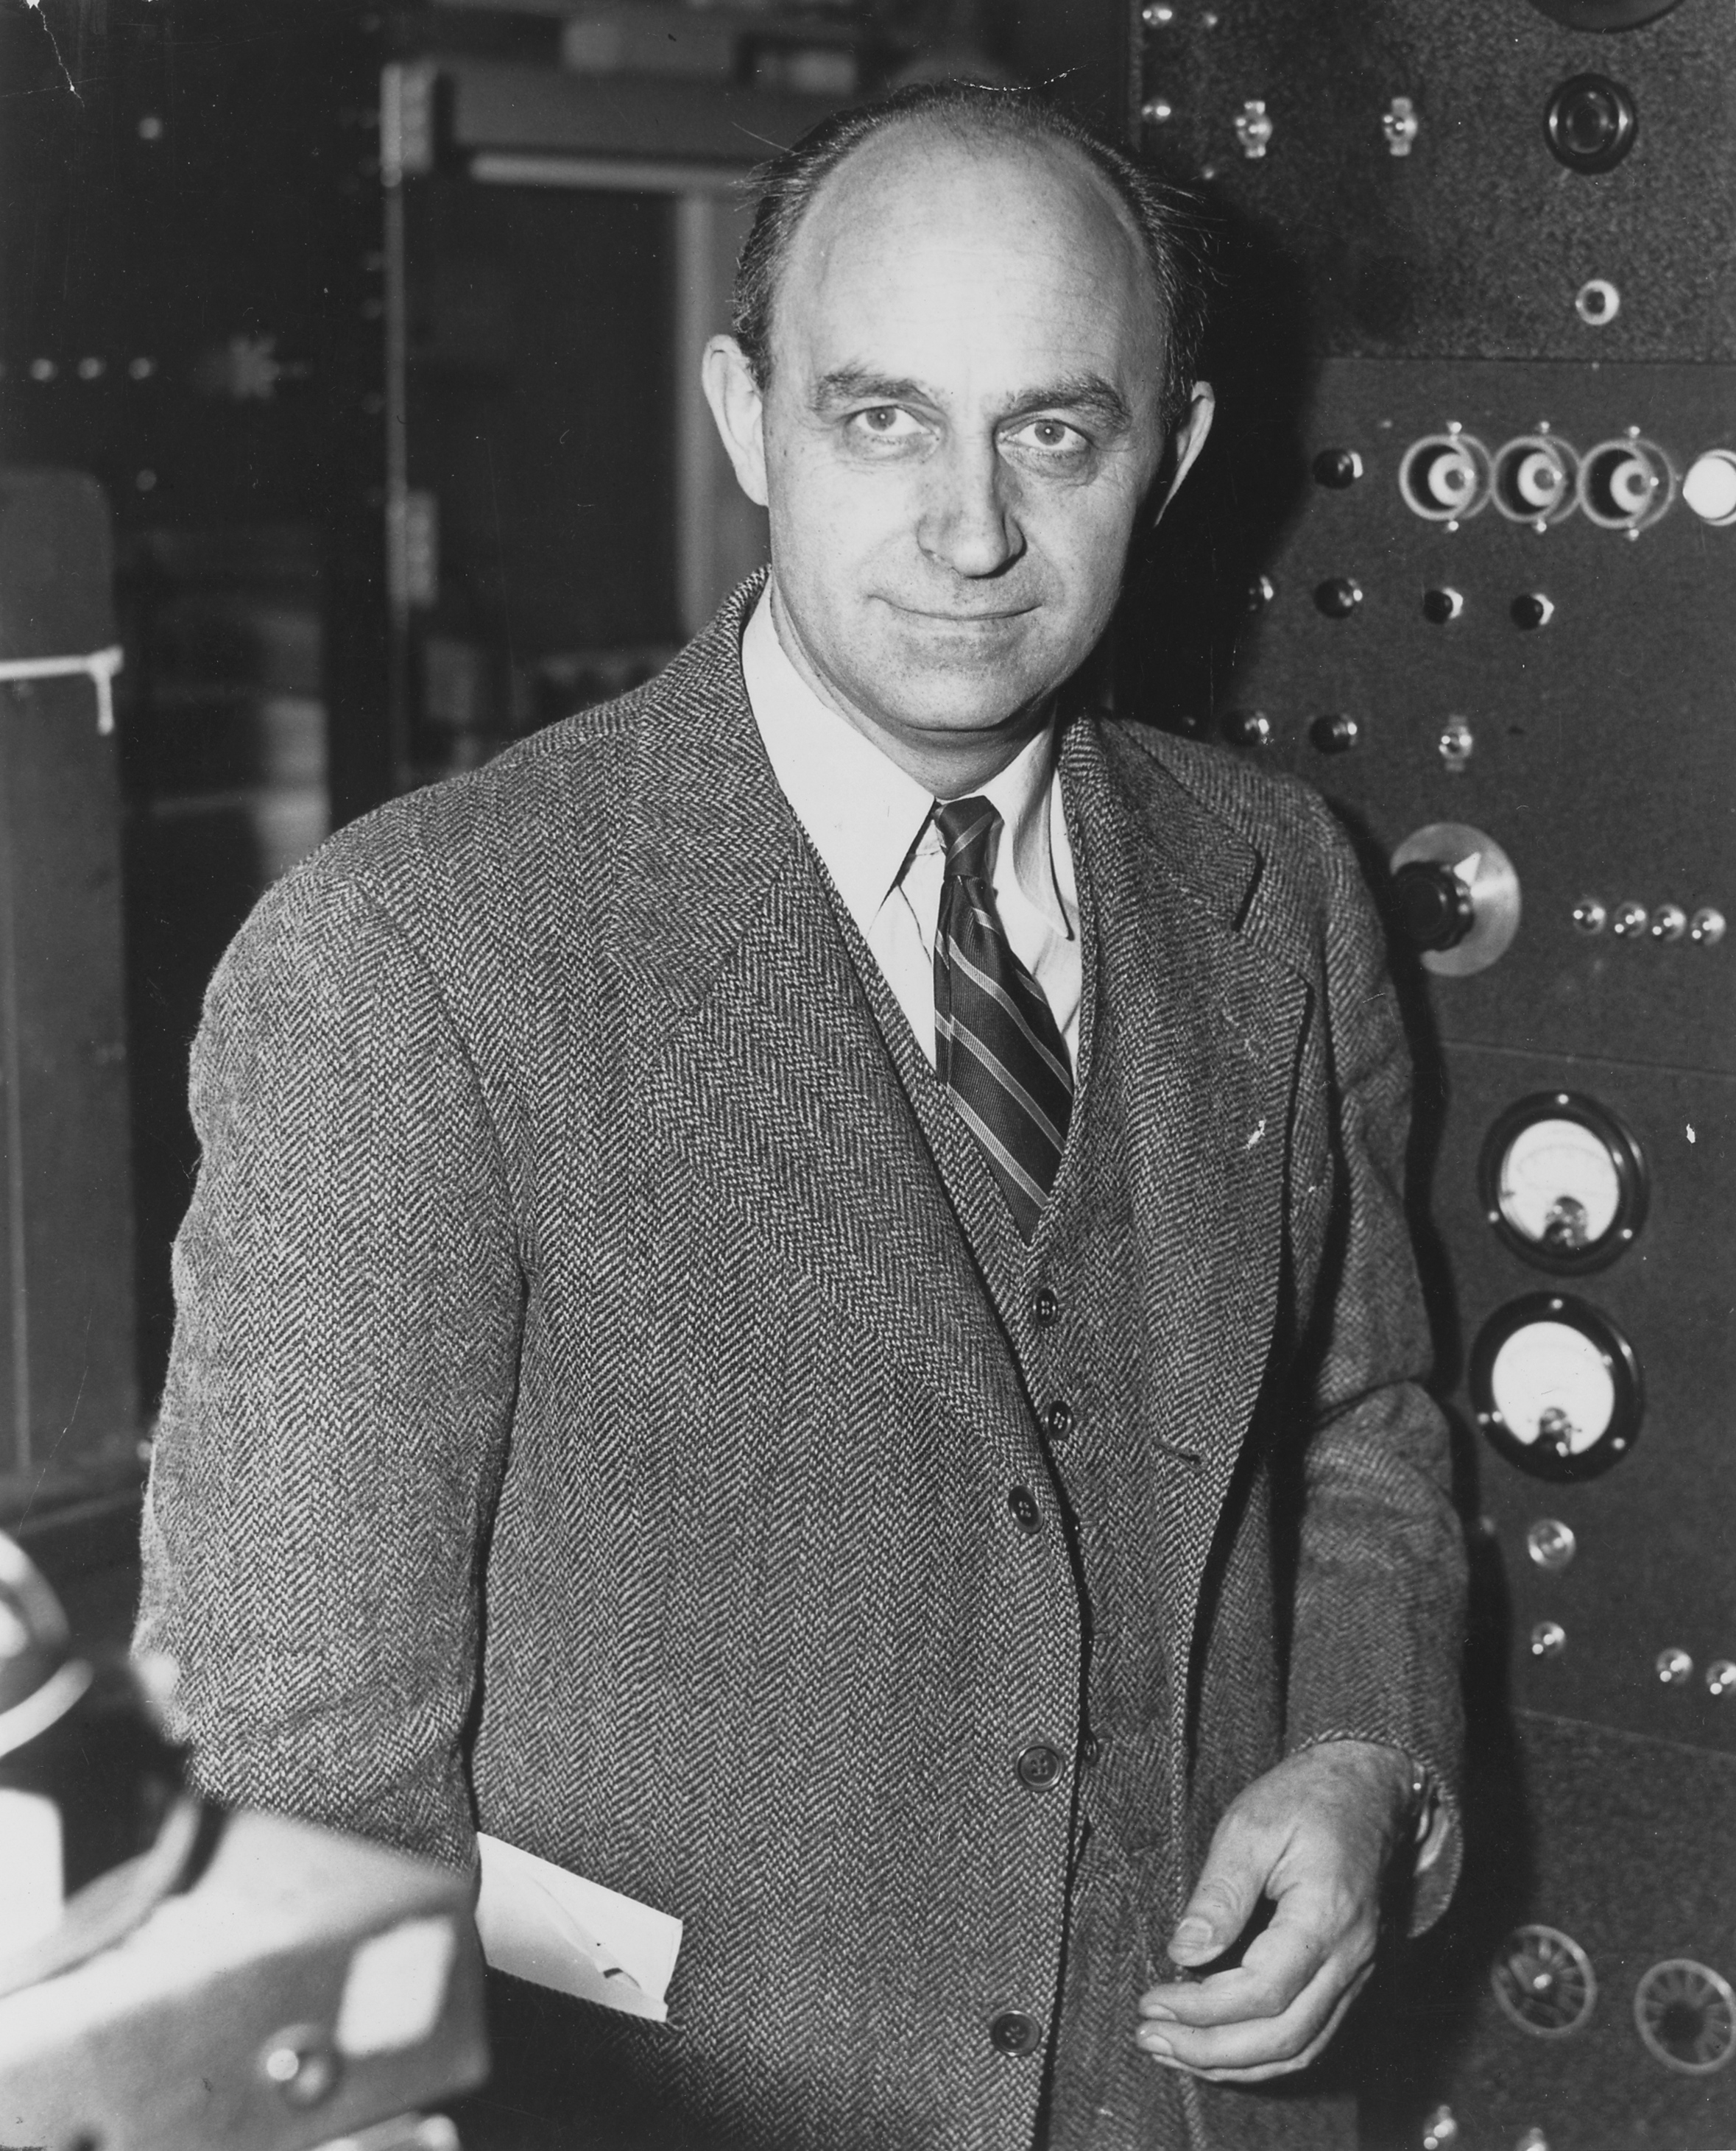
\includegraphics[width=\linewidth]{Images/Enrico_Fermi_1943-49.jpg}
	  			\caption{Enrico Fermi \cite{wiki:fermi}}
	  			\label{fig:fermi}
			\end{figure}
	\end{columns}
\end{frame}

\begin{frame}{Die elektroschwache Wechselwirkung}
	\begin{columns}
		\column{0.27\textwidth}
			\begin{figure}
	  			\centering
				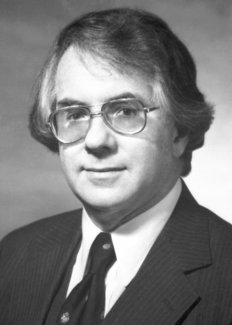
\includegraphics[width=\linewidth]{Images/glashow-13318-content-portrait-mobile-tiny.jpg}
	  			\caption{Sheldon Glashow}
	  			\label{fig:fermi}
			\end{figure}
				\column{0.27\textwidth}
			\begin{figure}
	  			\centering
				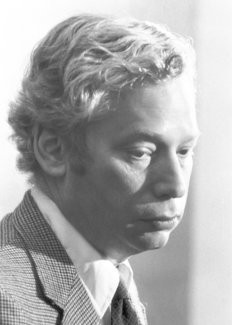
\includegraphics[width=\linewidth]{Images/weinberg-13320-content-portrait-mobile-tiny.jpg}
	  			\caption{Steven Weinberg}
	  			\label{fig:fermi}
			\end{figure}
				\column{0.27\textwidth}
			\begin{figure}
	  			\centering
				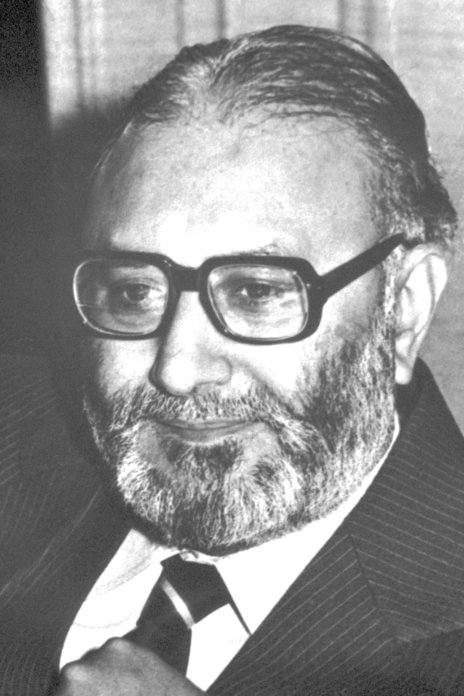
\includegraphics[width=\linewidth]{Images/salam-13319-portrait-mini-2x.jpg}
	  			\caption{Abdus Salam}
	  			\label{fig:fermi}
			\end{figure}
	\end{columns}
	\cite{9789810207274}
\end{frame}

\begin{frame}{Die elektroschwache Wechselwirkung}
			\begin{itemize}
				\setlength\itemsep{0.5em}
				\item \textbf{1968} wird die elektroschwache Wechselwirkung durch Sheldon Glashow, Steven Weinberg und Abdus Salam beschrieben
				\item Vereinheitlichte Theorie der Quantenelektrodynamik und schwachen Wechselwirkung
				\item Vier Austauschteilchen:
				\item [$\rightarrow$] Das masselose Photon $\gamma$
				\item [$\rightarrow$] Die massebehafteten Teilchen $W^+$, $W^-$, $Z^0$
				\item Geringe Stärke und Reichweite der schwachen Wechselwirkung wird begründet durch die hohen Massen der Austauschteilchen
				\item Schwacher Mischungswinkel $\Theta_\text{W}$ als freier Parameter
			\end{itemize}

\end{frame}


\section{Die Entdeckung der neutralen Ströme}

\begin{frame}{Neutrale Ströme (NC)}
	\begin{columns}
		\column{0.5\textwidth}
				\begin{itemize}
					  \setlength\itemsep{0.5em}
					\item Vorhersage der neutralen Ströme durch die elektroschwache Wechselwirkung
				\end{itemize}
				\vspace*{20px}
				\begin{itemize}
					\setlength\itemsep{0.5em}
					\item Leptonische NC: $\nu_\mu + e^- \rightarrow \nu_\mu + e^-$
					\item[$\rightarrow$] Signatur: Einzelnes Elektron
					\item Hadronische NC: $\nu_\mu + N \rightarrow \nu_\mu + X$
					\item[$\rightarrow$] Signatur: Nur Hadronen, ohne Leptonen
				\end{itemize}
		\column{0.5\textwidth}
			\begin{figure}
	  			\centering
				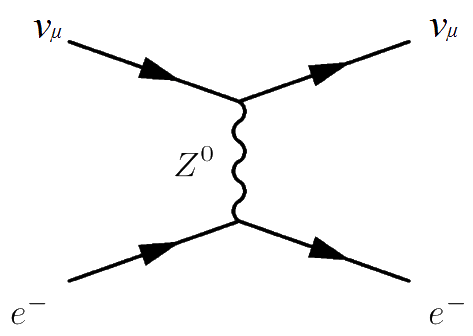
\includegraphics[width=\linewidth]{Images/Neutral_current,_leptonic_event,_muon_neutrino.png}
	  			\caption{Feynman-Diagramm eines leptonischen neutralen Stromes \cite{wiki:NC}}
	  			\label{fig:feynman}
			\end{figure}
	\end{columns}
\end{frame}


\begin{frame}{Der Gargamelle Detektor}
	\begin{columns}
		\column{0.6\textwidth}
				\begin{itemize}
					\setlength\itemsep{0.5em}
					\item Blasenkammer, betrieben am CERN von 1970 bis 1979
					\item[$\rightarrow$] Kammer gefüllt mit \SI{12}{\cubic\metre} Freon ($\ce{CBrF3}$)
					\item[$\rightarrow$] Temperatur der Flüssigkeit über der Siedetemperatur
					\item[$\rightarrow$] Durchquerende Teilchen ionisieren die Flüssigkeit, wobei Dampfblasen entstehen
					\item[$\rightarrow$] Nachweis der Gasblasen durch Kameras
					\item Kammer \SI{4.8}{\meter} lang, \SI{2}{\meter} im Durchmesser, \SI{2}{\tesla} Magnetfeld (zur Rekonstruktion)
				\end{itemize}

		\column{0.4\textwidth}
			\begin{figure}
	  			\centering
				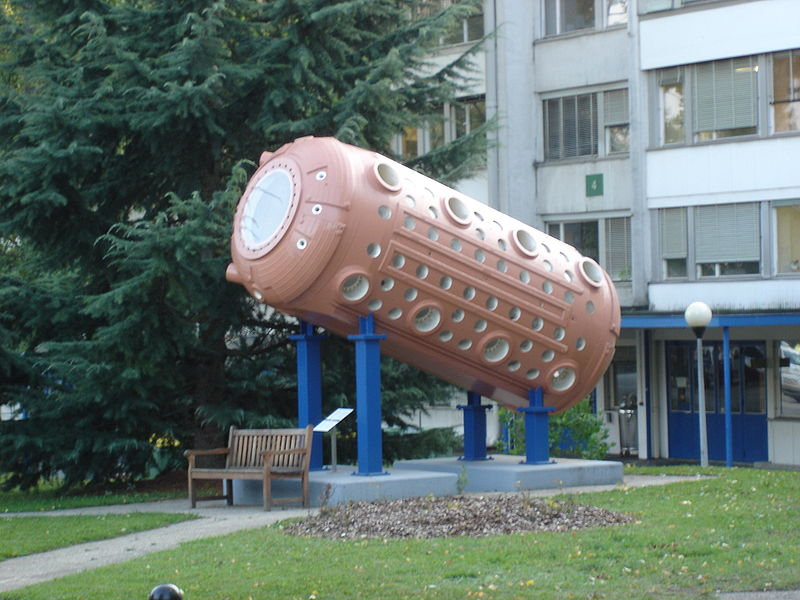
\includegraphics[width=\linewidth]{Images/800px-Gargamelle.jpg}
	  			\caption{Gargamelle Blasenkammer, ausgestellt am CERN \cite{wiki:gargamelle}}
	  			\label{fig:feynman}
			\end{figure}
	\end{columns}
\end{frame}

\begin{frame}
	\begin{figure}
	  \centering
	  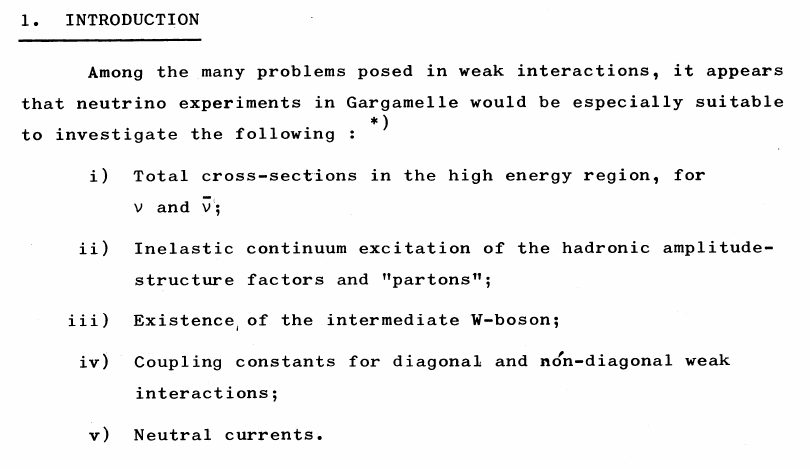
\includegraphics[width=0.9\linewidth]{Images/Screenshot_2018-11-26_16-27-27.png}
	  \caption{Auszug aus dem Proposal zum Gargamelle Detektor, März 1970 \cite{proposal}.}
	  \label{fig:proposal}
	\end{figure}
\end{frame}

\begin{frame}{Der Gargamelle Detektor - Neutrinoquelle}
	\begin{columns}
		\column{0.6\textwidth}
				\begin{itemize}
					\setlength\itemsep{0.5em}
					\item Als Neutrinoquelle diente ein Protonenbeam vom Proton Syncrotron (\SI{26}{\giga\electronvolt})
					\item[$\rightarrow$] Entstehung von Kaonen und Pionen durch Kollision der Protonen mit einem Beryllium-Target
					\item[$\rightarrow$] Kaonen und Pionen werden fokussiert und zerfallen in einem \SI{70}{\metre} langen Tunnel in Myonen und Neutrinos
					\item[$\rightarrow$] Neutrinoenergie im Bereich \SI{1}{\giga\electronvolt} bis \SI{10}{\giga\electronvolt}
				\end{itemize}

		\column{0.4\textwidth}
			\begin{figure}
	  			\centering
				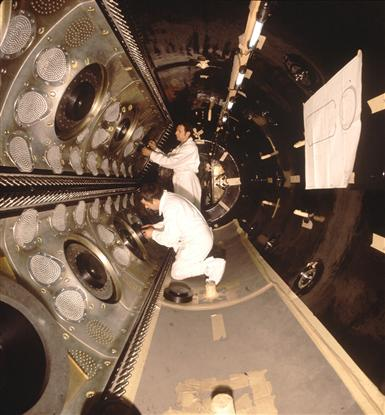
\includegraphics[width=\linewidth]{Images/7011042-A5-at-72-dpi.jpg}
	  			\caption{Blick in die Gargamelle Blasenkammer \cite{CERN-EX-7011042}}
	  			\label{fig:feynman}
			\end{figure}
	\end{columns}
\end{frame}

\begin{frame}{Der Gargamelle Detektor - Erste Resultate}
	\begin{columns}
		\column{0.6\textwidth}
				\begin{itemize}
					\setlength\itemsep{0.5em}
					\item \textbf{März 1972}: Erste Hinweise auf hadronische schwache Ströme ändern die Prioritäten der Analyse
					\item[$\rightarrow$] Suche sowohl nach hadronischen als auch leptonischen Events
					\item[$\rightarrow$] Leptonische Events: Weniger Hintergrundereignisse, treten jedoch selten auf
					\item \textbf{Dezember 1972}: Erste Beobachtung eines leptonischen NC-Events
					\item \textbf{19. Juli 1973}: Entdeckung der schwachen Ströme (leptonisch und hadronisch) wird präsentiert
				\end{itemize}

		\column{0.4\textwidth}
			\begin{figure}
	  			\centering
				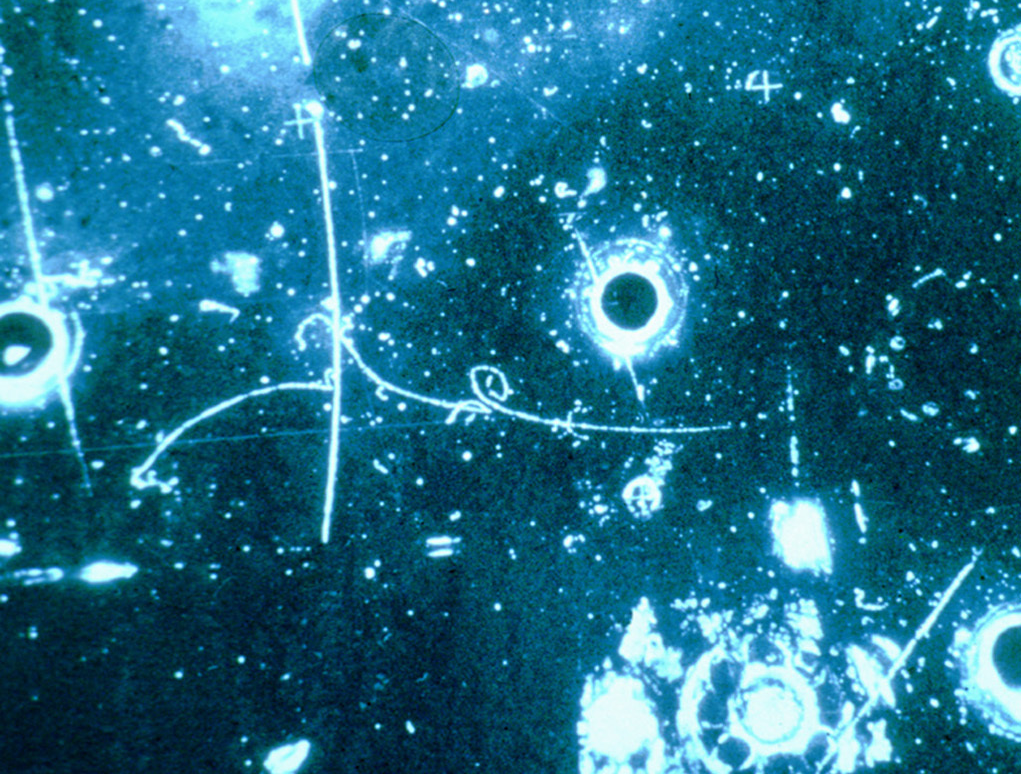
\includegraphics[width=\linewidth]{Images/60100_bearbeitet.png}
	  			\caption{Beobachtung eines leptonischen neutralen Stromes \cite{CERN-EX-60100}. Das Elektron bewegt sich horizontal von rechts nach links.}
	  			\label{fig:feynman}
			\end{figure}
	\end{columns}
\end{frame}

\begin{frame}{Der Gargamelle Detektor - Erste Resultate}
		\begin{itemize}
			\setlength\itemsep{0.5em}
			\item Aus den Ergebnissen des Experimentes konnten die Massen von W-Boson und Z-Boson vorhergesagt werden \cite{doi:10.1142/9789814644150_0006}:
			\begin{align*}
				M_\text{W} &\approx \left(60-80\right)\si{\giga\electronvolt}\\
				M_\text{Z} &\approx \left(75-92\right)\si{\giga\electronvolt}
			\end{align*}
			\item Jedoch existierte noch kein Experiment, welches die zur Erzeugung notwendige Schwerpunktsenergie zur Verfügung stellen konnte
			\item[$\Rightarrow$]Verschieben der "energy frontier" notwendig!

		\end{itemize}
\end{frame}

\section{"Pushing the energy frontier"}

\begin{frame}{Carlo Rubbia}
	\begin{columns}
		\column{0.6\textwidth}
				\begin{itemize}
					\setlength\itemsep{0.5em}
					\item Carlo Rubbia, geboren \textbf{1934} in Gorizia (Italien)
					\item Bereits früh ein Experte im Bereich der Elektronik
					\item Promovierte \textbf{1958} in Pisa und ging danach nach Columbia
					\item Ging nach wenigen Jahren zurück nach Europa zum CERN, bereits mit Mitte 20 "Group leader"
					\item Nimmt \textbf{1970} eine volle Professorenstelle in Harvard an
				\end{itemize}

		\column{0.4\textwidth}
			\begin{figure}
	  			\centering
				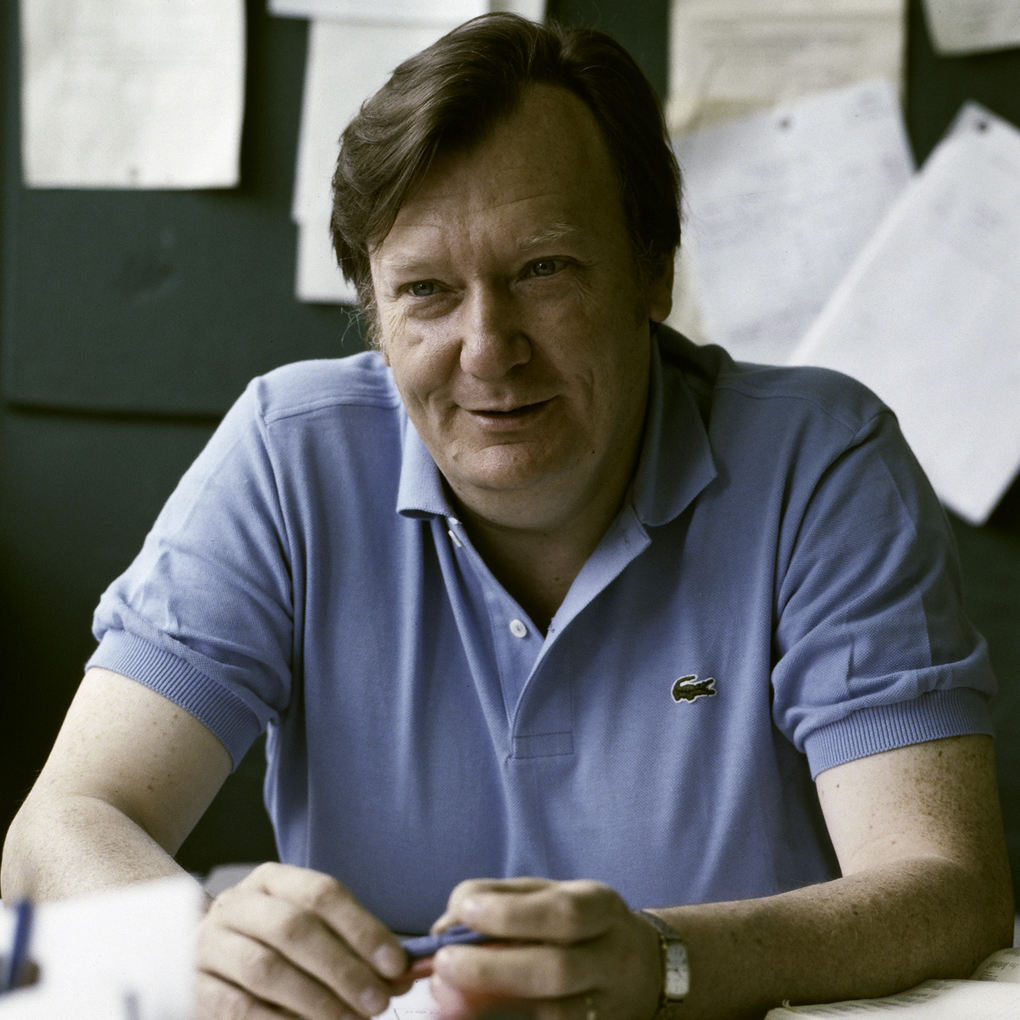
\includegraphics[width=\linewidth]{Images/8308555X.jpg}
	  			\caption{Carlo Rubbia im Jahre 1983 \cite{CERN-PHOTO-8308555}}
	  			\label{fig:feynman}
			\end{figure}
	\end{columns}
\end{frame}

\begin{frame}{Carlo Rubbia}
	\begin{columns}
		\column{0.6\textwidth}
				\begin{itemize}
					\setlength\itemsep{0.5em}
					\item Hatte häufig unendlich viele Ideen für Experimente, jedoch selten die Geduld, diese umzusetzen
					\item Keinen Ruf für genaue Analysen:\\
					\emph{"His numbers are what they are. They are usually wrong - but if they suit his purpose, nothing is wrong."} (Bernard Sadoulet, \cite{1556151128})
					\item Seine Expertise war in den 1970er Jahren zwar bekannt, jedoch auch seine Misserfolge
					\item[$\Rightarrow$] z.B. widersprachen seine Analysen zunächst der Existenz neutraler Ströme
				\end{itemize}

		\column{0.4\textwidth}
			\begin{figure}
	  			\centering
				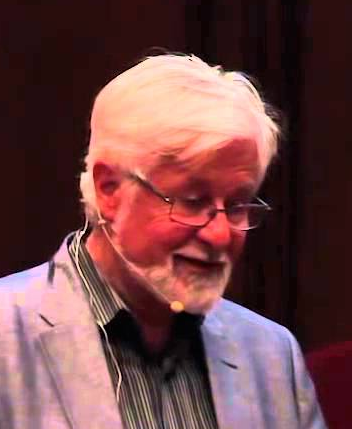
\includegraphics[width=0.8\linewidth]{Images/sadoulet.png}
	  			\caption{Bernard Sadoulet auf einer Konferenz in Amsterdam, 2013 \cite{Sadoulet}}
	  			\label{fig:sad}
			\end{figure}
	\end{columns}
\end{frame}

\begin{frame}{Super Proton Synchrotron}
	\begin{columns}
		\column{0.6\textwidth}
				\begin{itemize}
					\setlength\itemsep{0.5em}
					\item Super Proton Synchrotron (SPS) mit Umfang $R = \SI{6.9}{\kilo\meter}$ am CERN
					\item Ging \textbf{Juni 1976} in Betrieb
					\item Teilchenenergien von $E = \SI{400}{\giga\electronvolt}$ wurden erreicht
					\item Nutzung als fixed-target Experimenten mit Protonen:\\
					$\rightarrow$ $\sqrt{s} \approx \sqrt{2 \cdot E \cdot m} \approx \SI{27}{\giga\electronvolt} \ll M_W, M_Z$ 
					\item SPS wird bis heute als Vorbeschleuniger am LHC sowie für Experimente wie COMPASS, NA-61 und NA-62 genutzt
				\end{itemize}

		\column{0.4\textwidth}
			\begin{figure}
	  			\centering
				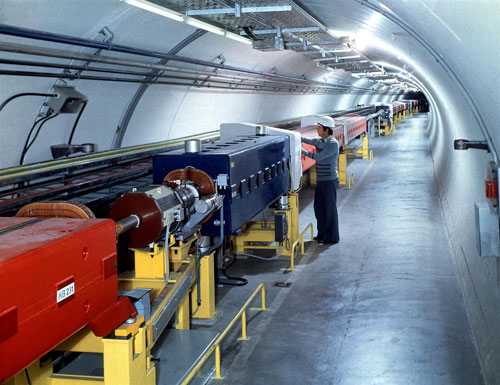
\includegraphics[width=\linewidth]{Images/sps.jpg}
	  			\caption{Super Proton Synchrotron (SPS) \cite{sps}}
	  			\label{fig:sad}
			\end{figure}
	\end{columns}
\end{frame}

\begin{frame}{Colliding-Beam-Experimente}
	\begin{columns}
		\column{0.5\textwidth}
				\begin{itemize}
					\setlength\itemsep{0.5em}
					\item Idee: Nutzung von Proton-Proton-Kollisionen (pp) um ausreichende Schwerpunktsenergien zu erreichen: \\
					\item[$\rightarrow$] Für Colliding-Beam-Experimente gilt $\sqrt{s} = 2 \cdot E$
					\item[$\rightarrow$] Unter Berücksichtigung der Partonstruktur $\sqrt{s} = 2 \cdot E \cdot x$ (mit $x \approx 0.2$)
					\item Hierdurch wären geringere Teilchenenergien notwendig
				\end{itemize}

		\column{0.5\textwidth}
			\begin{figure}
	  			\centering
				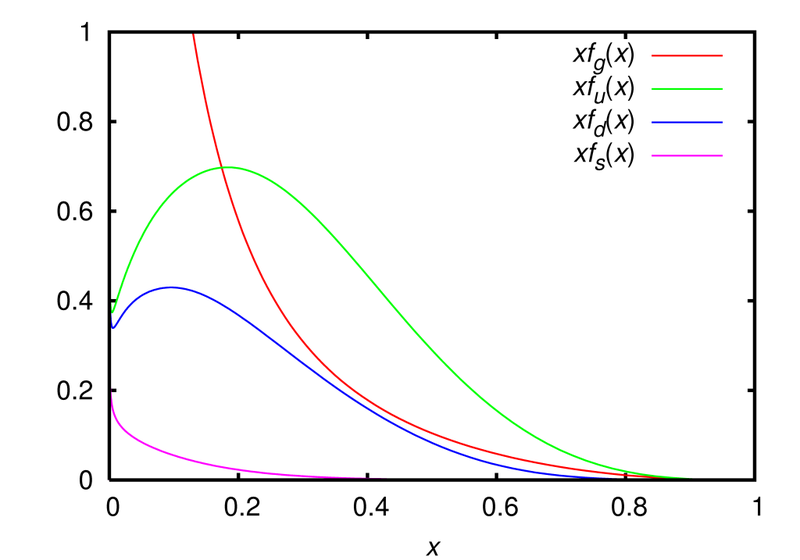
\includegraphics[width=\linewidth]{Images/pdf.png}
	  			\caption{Partonverteilungsfunktion für das Proton, wobei $x$ den Impulsanteil der Partons am gesamten Proton angibt. Die y-Achse ist proportional zur Wahrscheinlichkeit für das jeweilige $x$ \cite{wiki:pdf}.}
	  			\label{fig:sad}
			\end{figure}
	\end{columns}
\end{frame}

\begin{frame}{Colliding-Beam-Experimente}
	\begin{columns}
		\column{0.6\textwidth}
				\begin{itemize}
					\setlength\itemsep{0.5em}
					\item \textbf{Januar 1975}: Workshop am Fermilab, um über die Möglichkeiten von pp-Experimenten zu sprechen
					\item Vortrag des jungen Peter M. McIntyre, Kollisonen von Protonen und Antiprotonen durchzuführen
					\item[$\rightarrow$] Protonen und Antiprotonen könnten sich im selben Rohr befinden und die gleichen Magneten nutzen
					\item[$\rightarrow$] Umbau eines bestehenden Proton-Synchrotrons wäre ausreichend
					\item[$\rightarrow$] Herausforderung: Erzeugung der Antiprotonen in ausreichender Zahl sowie Kühlung
					\item Rubbia war, im Gegensatz zu den meisten Workshopteilnehmern, begeistert von der Idee
				\end{itemize}
		\column{0.4\textwidth}
			\begin{figure}
	  			\centering
				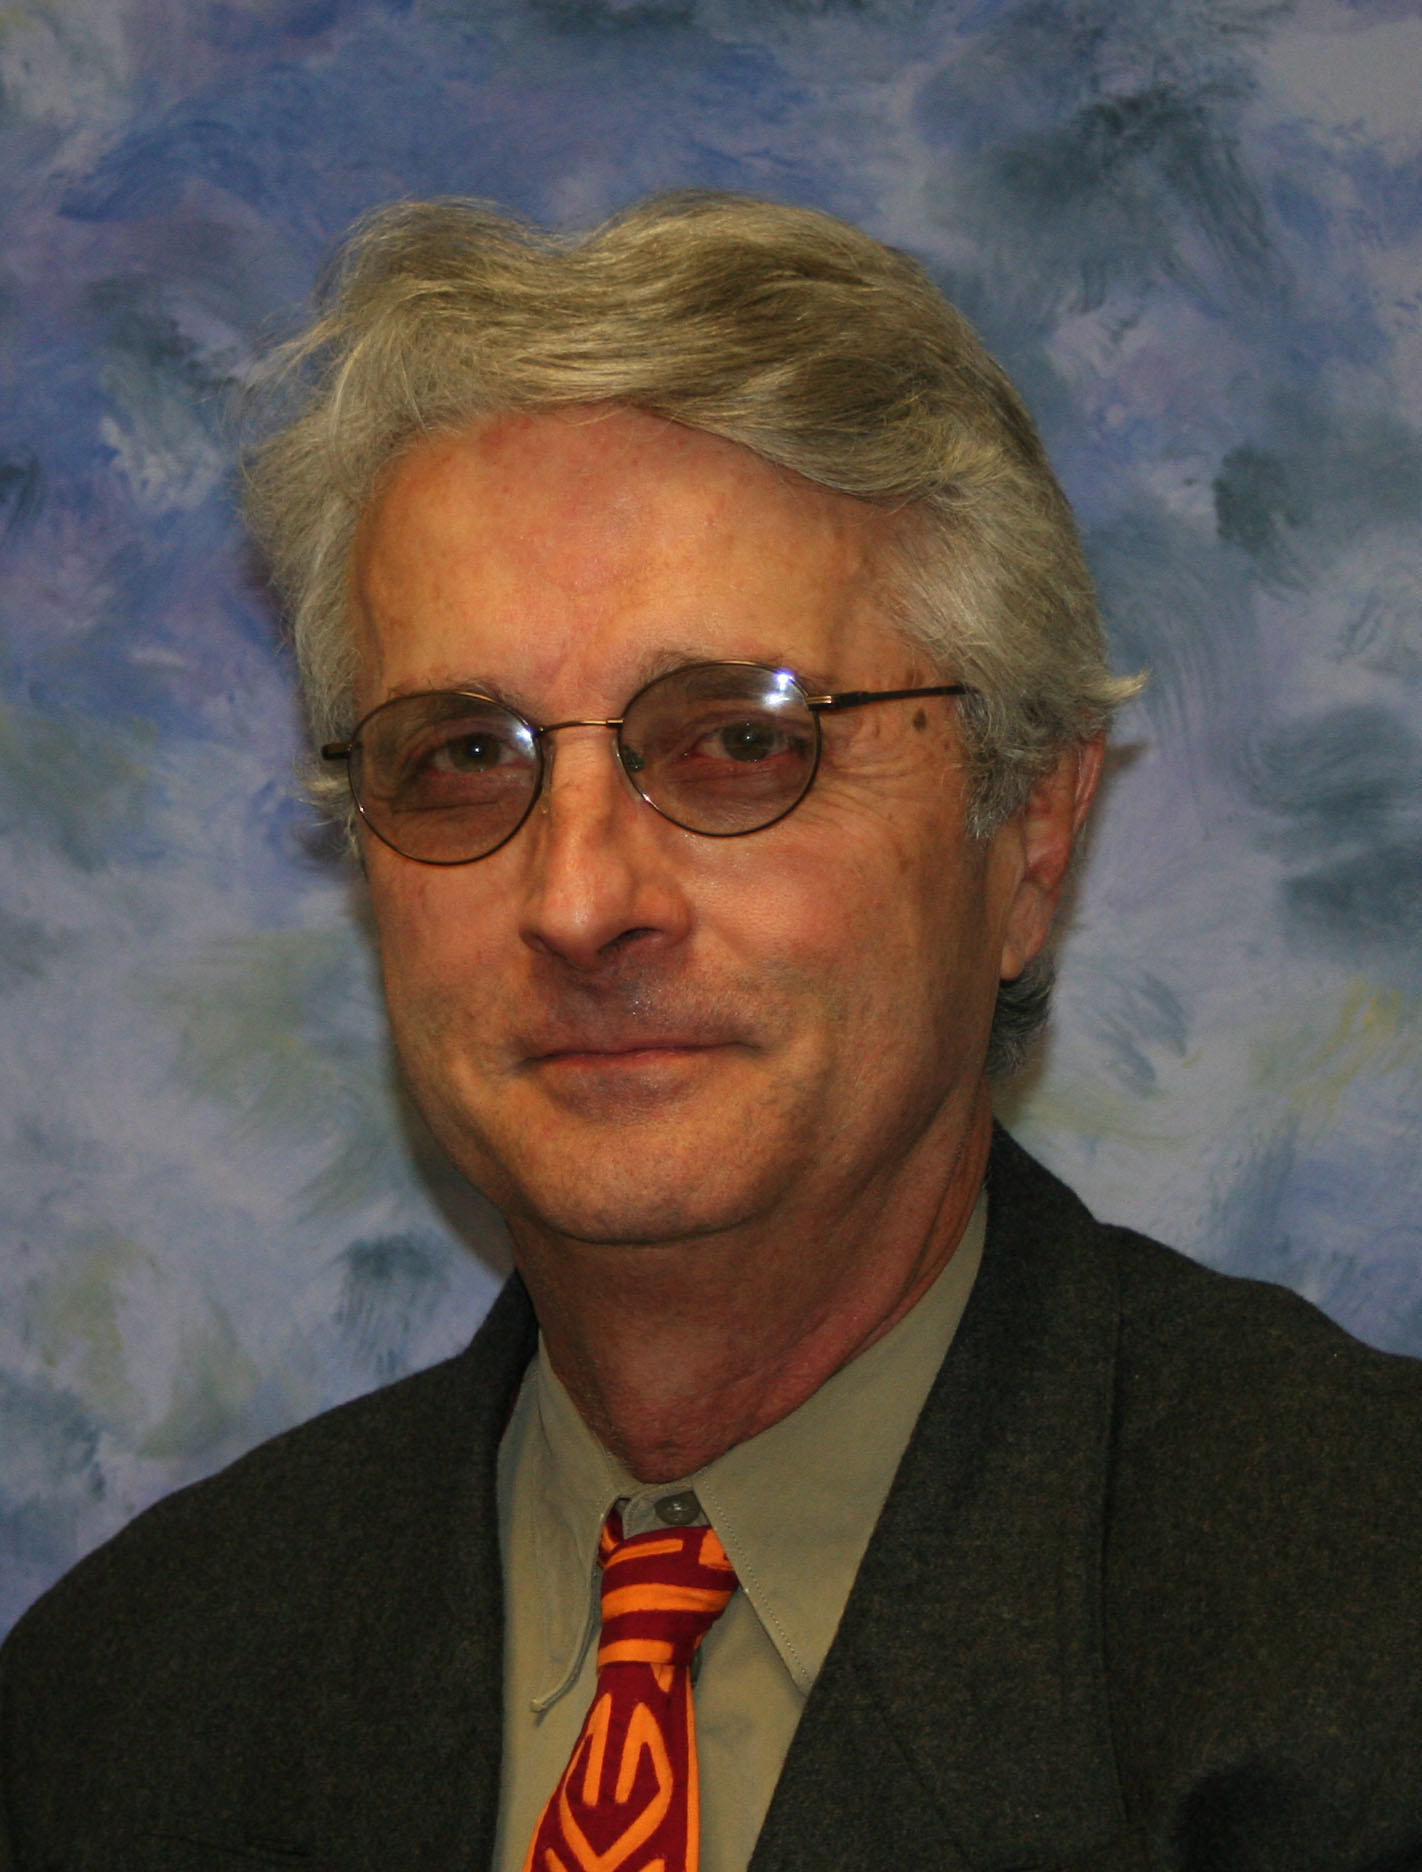
\includegraphics[width=0.8\linewidth]{Images/mcintyre.jpg}
				\caption{Peter M. McIntyre \cite{mci}}
	  			\label{fig:sad}
			\end{figure}

	\end{columns}
\end{frame}

\begin{frame}{Die Misere des CERNs}
				\begin{itemize}
					\setlength\itemsep{0.5em}
					\item In den vergangenen 25 Jahren gab es keine bedeutende Entdeckungen am CERN oder Nobelpreise
					\item[$\rightarrow$] $J/\Psi$-Entdeckung am CERN wurde verpasst
					\item[$\rightarrow$] Keinen Nobelpreis für die neutralen Ströme
					\item Experimente die am CERN abgelehnt wurden, haben häufig an anderen Standorten Entdeckungen gebracht
				\end{itemize}
				\vspace*{10px}
				\begin{itemize}
					\item[$\rightarrow$] Das CERN war bestrebt, eine neue Entdeckung zu machen
				\end{itemize}
\end{frame}

\begin{frame}{Umbau des SPS in einen Proton-Antiproton-Collider}
				\begin{itemize}
					\setlength\itemsep{0.5em}
					\item Rubbia und McIntyre schlug dem CERN \textbf{1976} vor, den vorhandenen Beschleuniger SPS in einen Proton-Antiproton-Collider umzubauen
					\item[$\rightarrow$] Mit einer Strahlenergie von $E = \SI{300}{\giga\electronvolt}$ könnte eine Schwerpunktsenergie von $\sqrt{s} = 2 \cdot E \cdot x = \SI{120}{\giga\electronvolt} > M_W, M_Z$ erreicht werden
					\item Bau des Eletron-Positron-Colliders (LEP) war geplant, würde aber noch viele Jahre dauern
					\item Geld war vorhanden, und die Chance auf die Entdeckung wäre sehr gut
				\end{itemize}
					\vspace*{10px}
				\begin{itemize}
					\item[$\Rightarrow$] \textbf{Januar 1978}: Bestätigung des CERNs, den SPS zum Super Proton Antiproton Synchrotron (Sp$\overline{\text{p}}$S) umzubauen
				\end{itemize}
\end{frame}

\begin{frame}{Das Super Proton Antiproton Synchrotron}
				\begin{itemize}
					\setlength\itemsep{0.5em}
					\item Betrieb von \textbf{Juli 1981} bis \textbf{1991}
					\item Speicherring für Protonen und Antiprotonen, Speicherzeit von 15 bis 20 Stunden
					\item Betrieb eines Speicherrings (Sp$\overline{\text{p}}$S) anspruchsvoller als der eines Synchrotrons (SPS)
					\item[$\rightarrow$] Bau einer beam line für entgegengesetzte Injektion
					\item[$\rightarrow$] Verbesserung des Vakuums um drei Grö{\ss}enordnungen
					\item[$\rightarrow$] Anpassung der Kavitäten, um p und $\overline{\text{p}}$ in exakten Bunches zu beschleunigen (so dass Kollsionen nur in den Detektoren stattfinden)
				\end{itemize}
\end{frame}

\begin{frame}{Betrieb des Sp$\overline{\text{p}}$S}
	\begin{columns}
		\column{0.6\textwidth}
				\begin{itemize}
					\setlength\itemsep{0.5em}
					\item Nachweis des Z-Bosons über Reaktion $\text{Z} \rightarrow e^+ e^-$
					\item[$\rightarrow$] Um mit dieser Reaktion eine Rate von 1 event pro Tag zu erreichen werden $\approx \num{3e10}$ Antiprotonen benötigt
					\item Protonen werden vom Proton Synchrotron (PS) auf $\SI{26}{\giga\electronvolt}$ beschleunigt und auf ein Target geleitet
					\item Entstehende Antiprotonen mit Impuls $\SI{3.5}{\giga\electronvolt}$ werden mit Spektrometer ausgewählt und an einen Speicherring, den Antiproton Accumulator (AA), weitergeleitet 
					\item[$\rightarrow$] Problem: Phasenraumvolumen der Antiprotonen
				\end{itemize}
		\column{0.4\textwidth}
			\begin{figure}
	  			\centering
				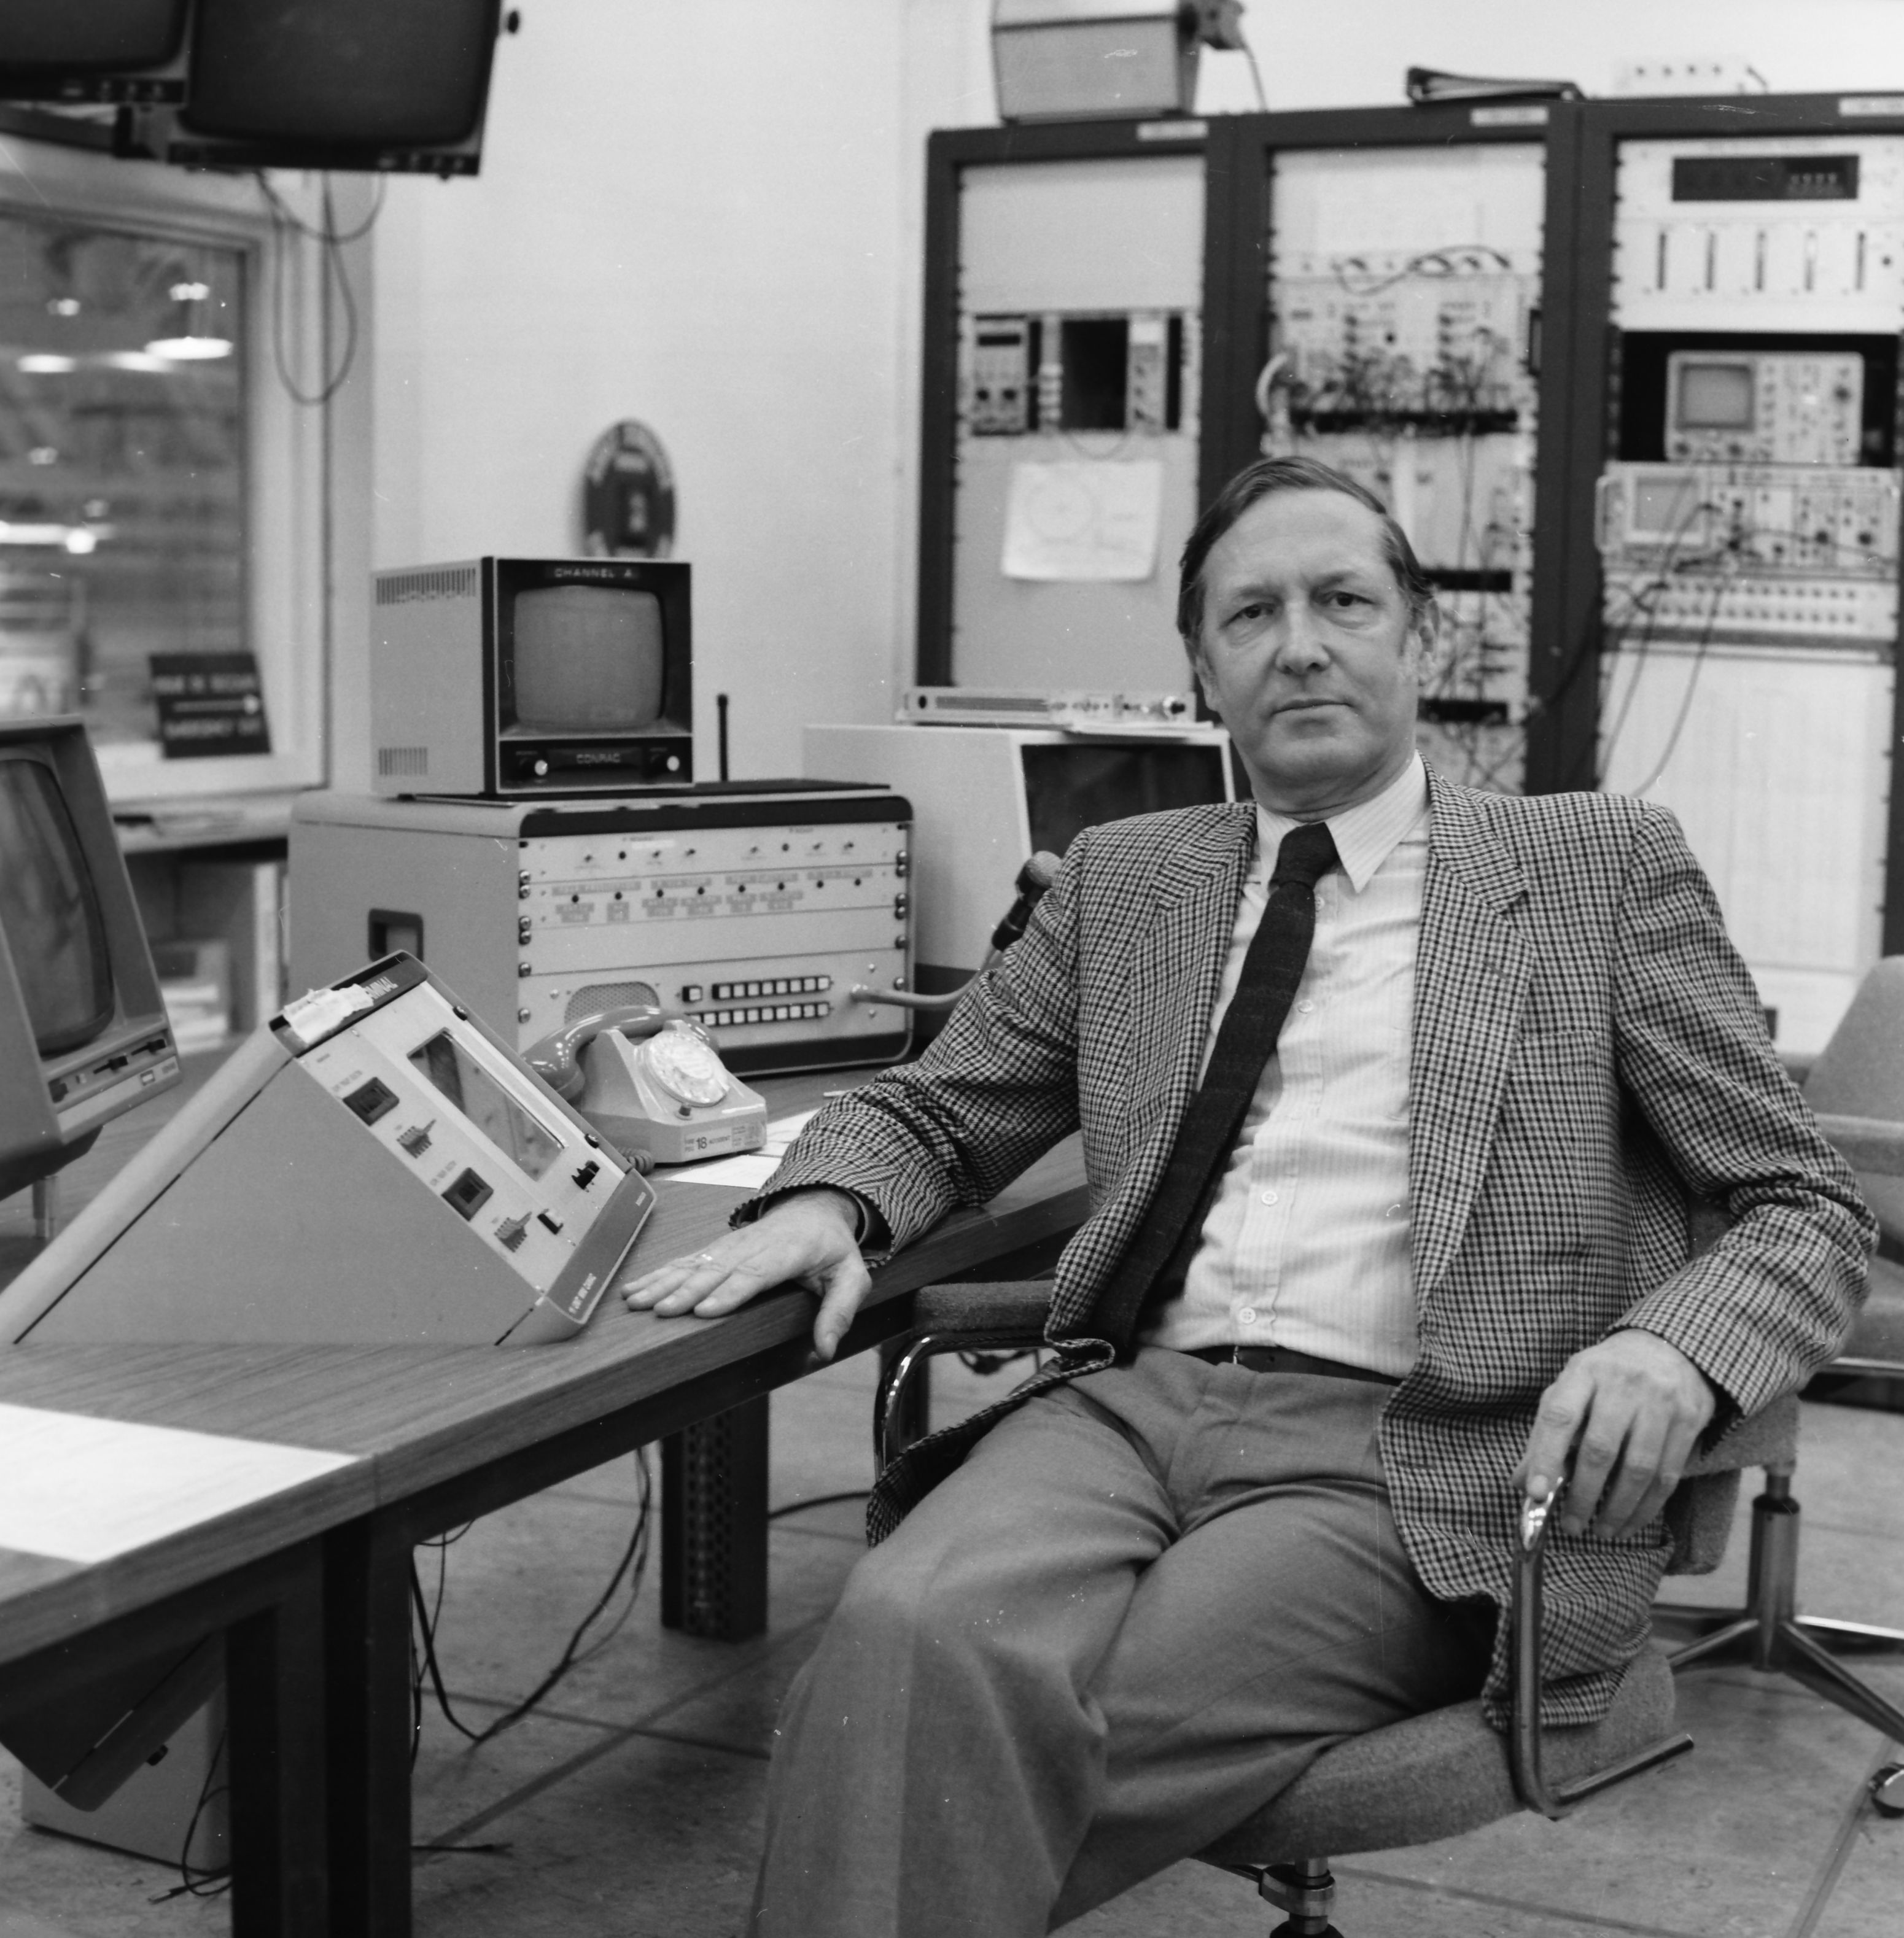
\includegraphics[width=\linewidth]{Images/8401333.jpg}
				\caption{Simon van der Meer im AA Kontrollraum \cite{CERN-PHOTO-8401333}}
	  			\label{fig:sad}
			\end{figure}
	\end{columns}
\end{frame}

\begin{frame}{Betrieb des Sp$\overline{\text{p}}$S - Stochastische Kühlung}
	\begin{columns}
		\column{0.65\textwidth}
				\begin{itemize}
					\setlength\itemsep{0.5em}
					\item Prinzip der stochastischen Kühlung: 1972 von Simon van der Meer entwickelt
					\item Ziel: Verringerung des Phasenraumvolumens im AA
					\item Teilchen, die von idealer Bahn im Speicherring abweichen, führen Oszillationen aus
					\item \textbf{Pick-up}: Messe Auslenkungen der Teilchen(gruppen) von Idealbahn\\
					$\rightarrow$ Ausgabe eines Signales proportional zu dieser Auslenkung
					\item \textbf{Kicker}: Wenn Teilchen Kicker passiert, führe über elektromagnetische Felder einen Korrektur durch
					\item Phasenraumverdichtung um Faktor $\num{1e9}$ ermöglicht
				\end{itemize}
		\column{0.35\textwidth}
			\begin{figure}
	  			\centering
				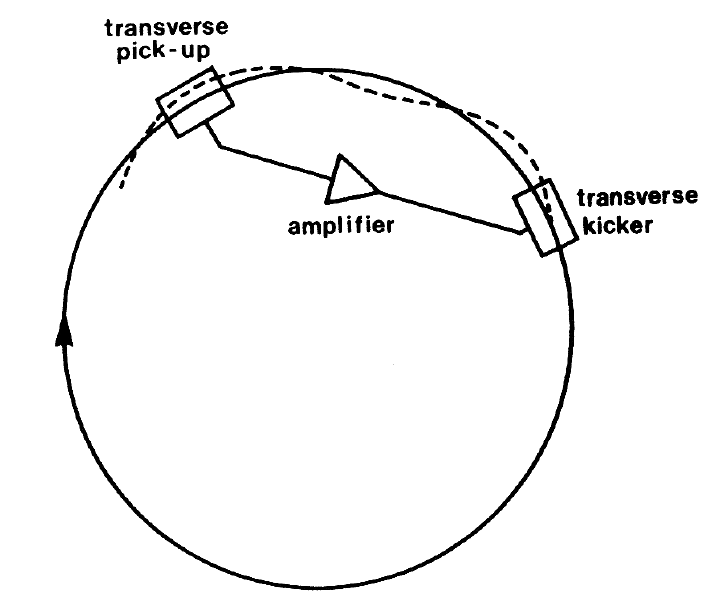
\includegraphics[width=\linewidth]{Images/Screenshot_2018-12-04_12-28-18.png}
				\caption{Prinzip der stochastischen Kühlung \cite{doi:10.1142/9789814644150_0006}}
	  			\label{fig:sad}
			\end{figure}
	\end{columns}
\end{frame}

\begin{frame}{Betrieb des Sp$\overline{\text{p}}$S}
				Sobald genug Antiprotonen im AA angesammelt:
				\begin{itemize}
					\setlength\itemsep{0.5em}
					\item Beschleunige drei Bunches an Protonen im SPS auf \SI{26}{\giga\electronvolt}
					\item[$\rightarrow$] Injektion der Protonen in den Sp$\overline{\text{p}}$S
					\item Führe Antiprotonen in SPS über, beschleunige sie in drei Bunches auf \SI{26}{\giga\electronvolt}
					\item[$\rightarrow$] Injektion der Antiprotonen in den Sp$\overline{\text{p}}$S in entgegengesetzte Richtung
					\item Beschleunigung im SPS auf bis zu \SI{315}{\giga\electronvolt}
					\item[$\rightarrow$] Ca. 15 bis 20 Stunden Datennahme möglich
				\end{itemize}

\end{frame}

\section{Die Suche nach den W- und Z-Bosonen}

\begin{frame}{Die Experimente am Sp$\overline{\text{p}}$S}
	\begin{columns}
		\column{0.6\textwidth}
				\begin{itemize}
					\setlength\itemsep{0.5em}
					\item Bewilligung der Experimente UA1 (Juni 1978) und UA2 (Ende 1978) am Sp$\overline{\text{p}}$S
					\item[$\rightarrow$] Beide mit dem Ziel, die W- und Z-Bosonen zu finden
					\item Experimente am Sp$\overline{\text{p}}$S lagen ca. \SI{50}{\metre} unter der Erde, deshalb die Namen \textbf{U}nderground \textbf{A}rea
					\item W-Boson zerfällt primär ($\approx \SI{70}{\percent}$) in ein Quark-Antiquark-Paar, welche als zwei hadronische Jets sichtbar wären
					\item[$\rightarrow$] Überlagert durch Untergrund aufgrund von harter Streuung der Partonen
					\item[$\rightarrow$] Stattdessen Nachweis des W-Bosons über die Signatur $\text{W} \rightarrow \text{l} \nu_\text{l}$
				\end{itemize}
		\column{0.4\textwidth}
			\begin{figure}
	  			\centering
				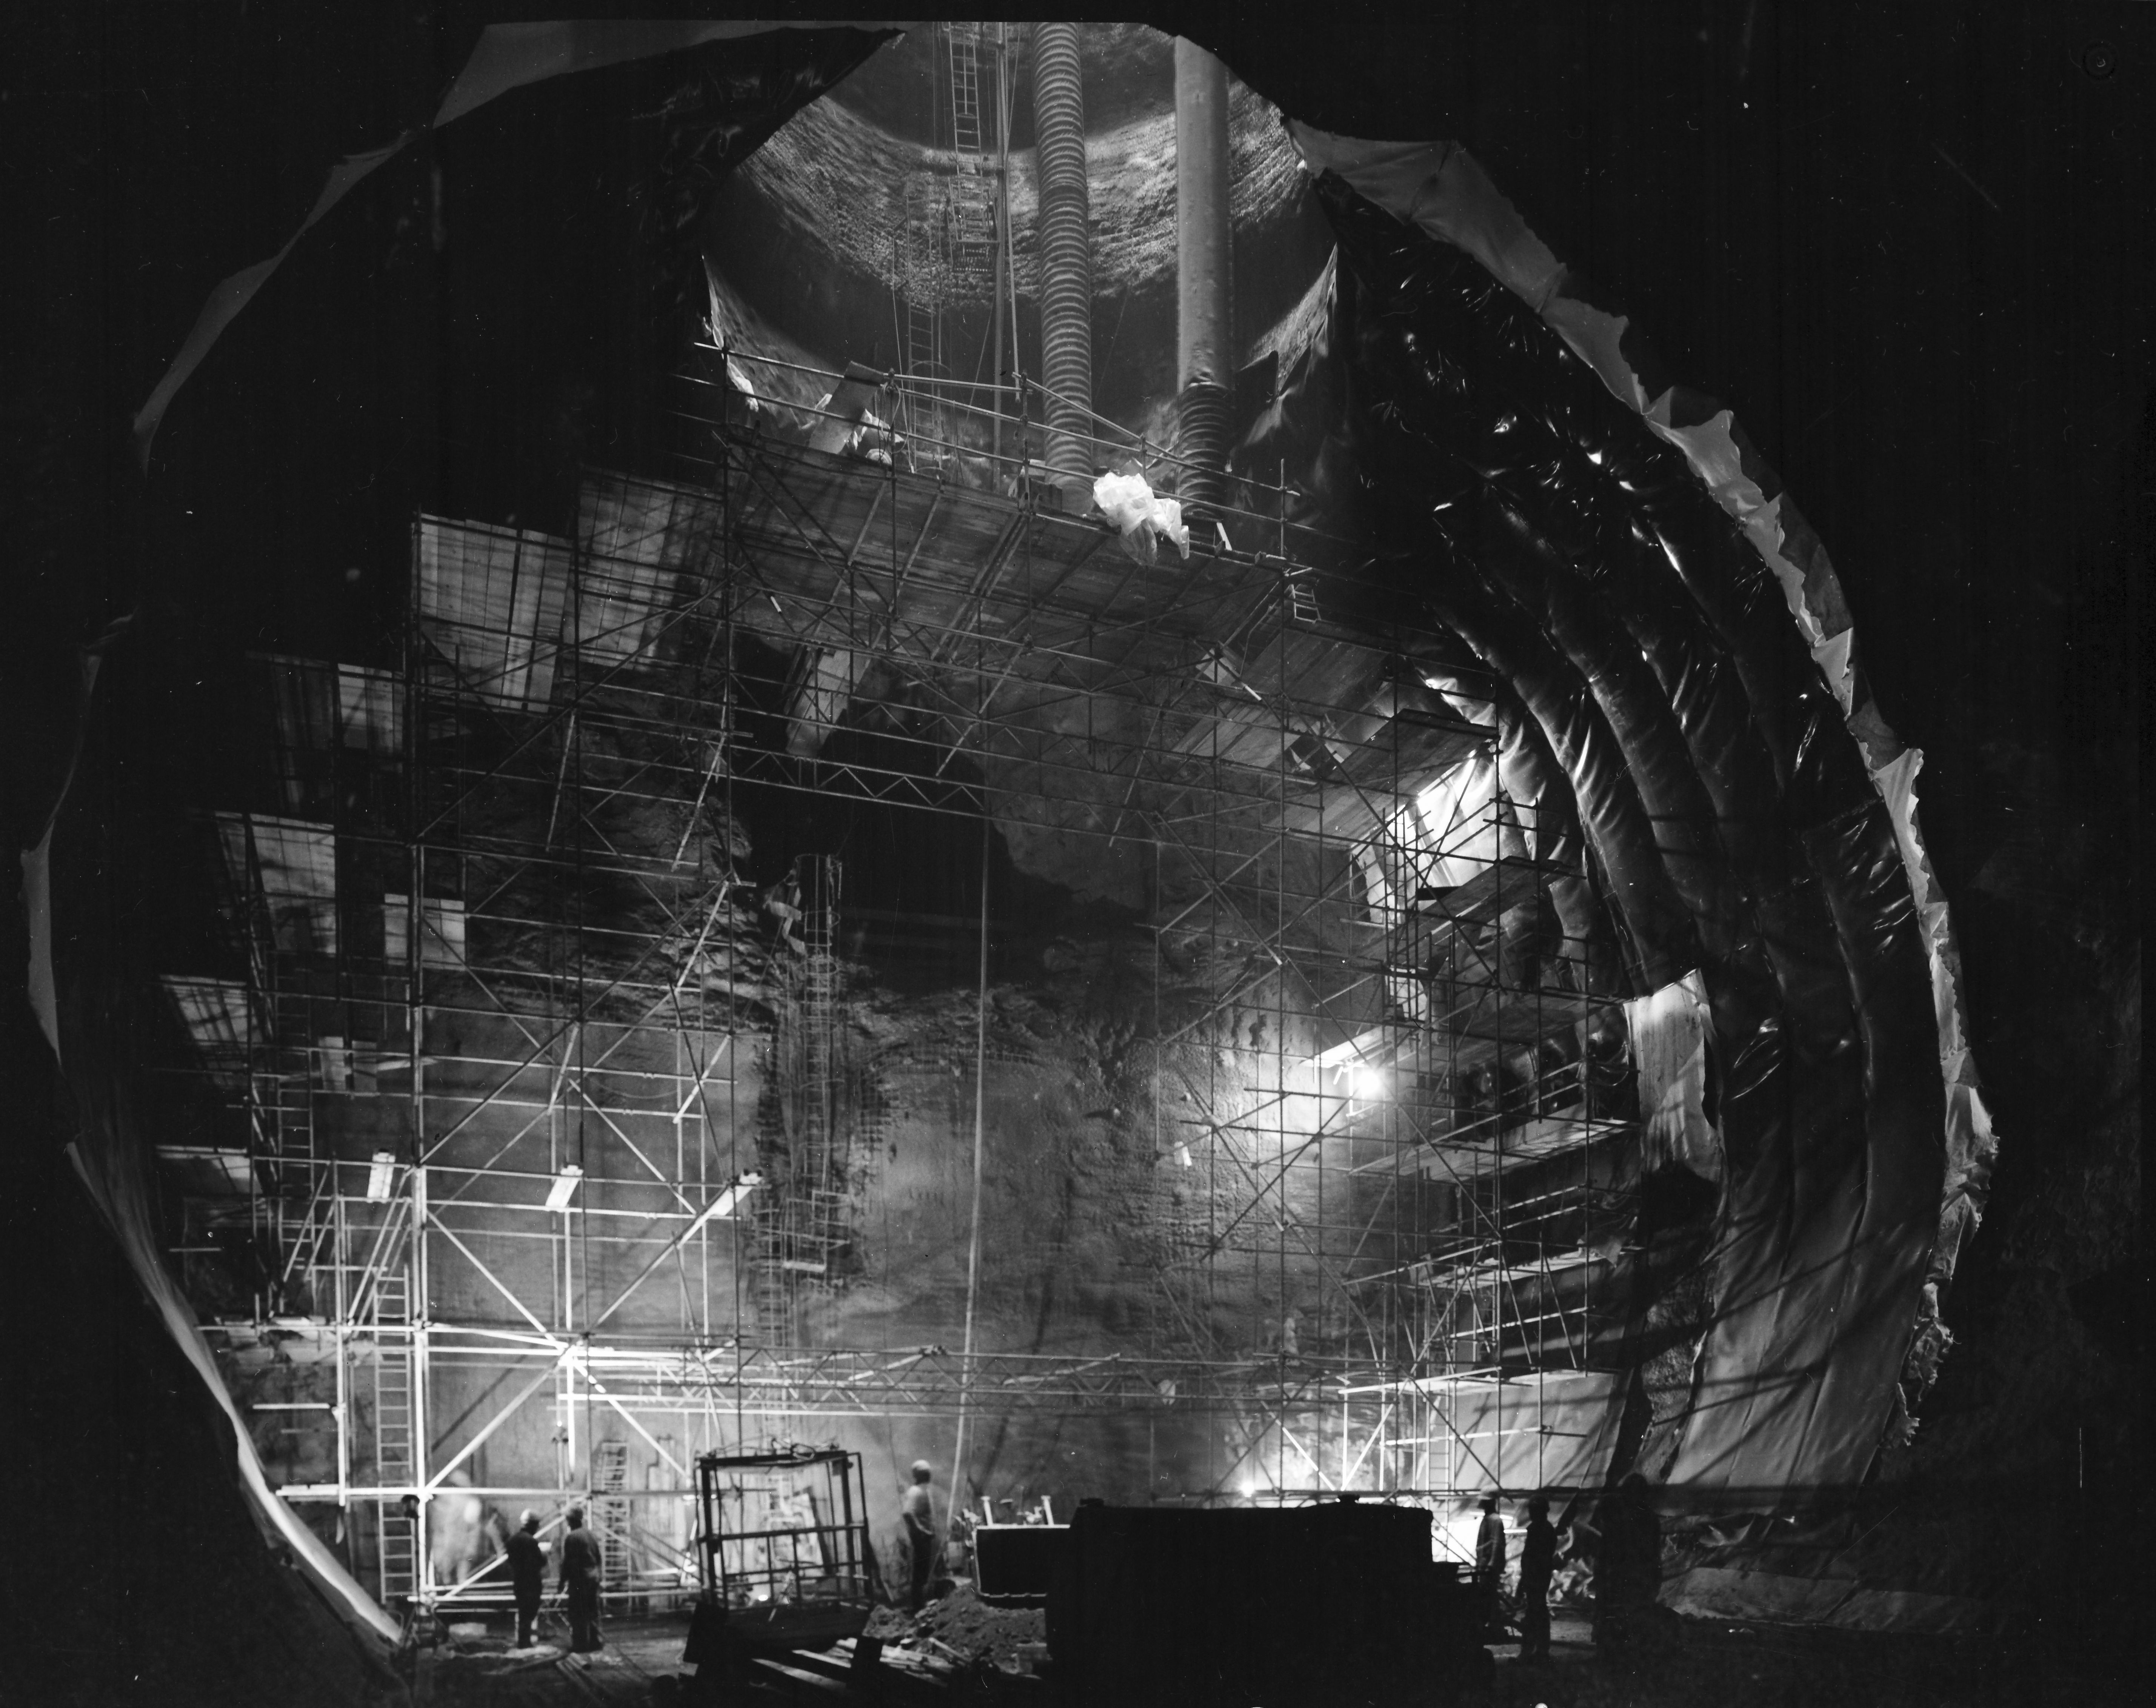
\includegraphics[width=\linewidth]{Images/8002262.jpg}
				\caption{Ausbau der Experimentierhalle für UA2, 1980 \cite{CERN-PHOTO-8002262}}
	  			\label{fig:sad}
			\end{figure}
	\end{columns}
\end{frame}

\begin{frame}{Die Experimente am Sp$\overline{\text{p}}$S - UA1}
	\begin{columns}
		\column{0.5\textwidth}
				\begin{itemize}
					\setlength\itemsep{0.5em}
					\item Team von ca. 130 Physikern, unter Leitung von Rubbia, arbeiteten an UA1
					\item Design: Gro{\ss}er, komplexer, multifunktionaler 4\pi-Detektor
					\item Umgeben von gro{\ss}em Dipolmagnet mit $\SI{0.7}{\tesla}$ Magnetfeld
					\item Driftkammer zur Rekonstruktion der Teilchenbahn, Energieverlust, Ladung und Impuls
				\end{itemize}
		\column{0.5\textwidth}
			\begin{figure}
	  			\centering
				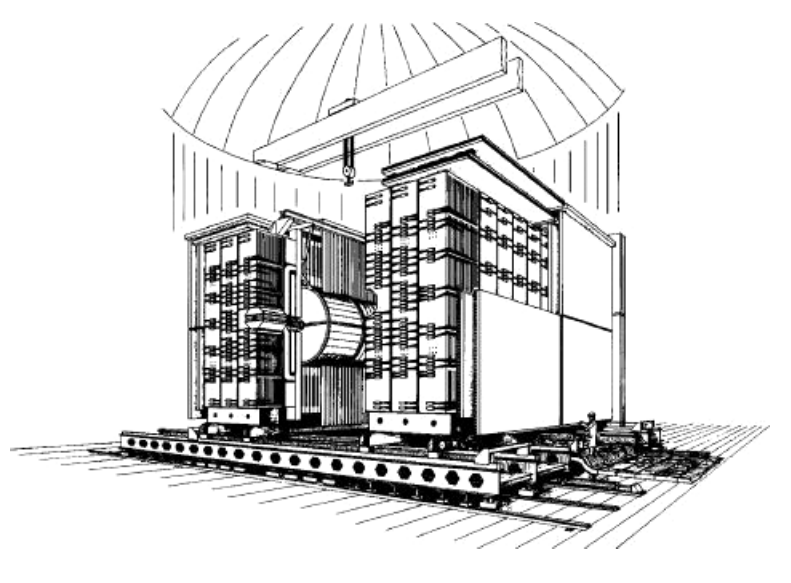
\includegraphics[width=\linewidth]{Images/Screenshot_2018-12-04_16-44-02.png}
				\caption{Skizze des Aufbaus von UA1 \cite{doi:10.1142/9789814644150_0006}. Der Detektor ist auseinandergefahren. }
	  			\label{fig:sad}
			\end{figure}
	\end{columns}
\end{frame}

\begin{frame}{Die Experimente am Sp$\overline{\text{p}}$S - UA1}
	\begin{columns}
		\column{0.5\textwidth}
				\begin{itemize}
					\setlength\itemsep{0.5em}
					\item Elektromagnetisches und hadronisches Kalorimeter
					\item[$\rightarrow$] Hermetisch abgeschlossen, um fehlenden transversalen Impuls rekonstruieren zu können
					\item[$\rightarrow$] Elektromagnetisches Kalorimeter abwechselnd aus Blei- und Szintillatorschichten (Sandwich-Kalorimeter)
					\item Myonkammern aus Driftröhren
				\end{itemize}
		\column{0.5\textwidth}
			\begin{figure}
	  			\centering
				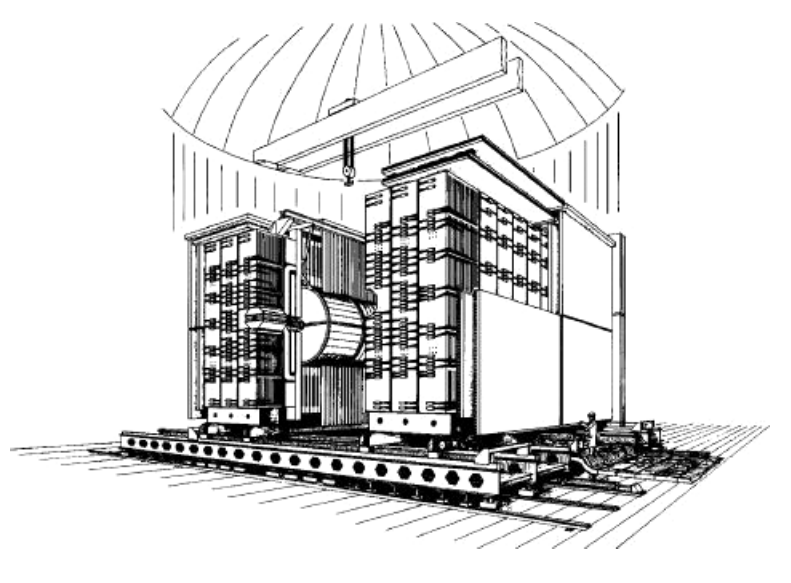
\includegraphics[width=\linewidth]{Images/Screenshot_2018-12-04_16-44-02.png}
				\caption{Skizze des Aufbaus von UA1 \cite{doi:10.1142/9789814644150_0006}. Der Detektor ist auseinandergefahren. }
	  			\label{fig:sad}
			\end{figure}
	\end{columns}
\end{frame}

\begin{frame}{Die Experimente am Sp$\overline{\text{p}}$S - UA2}
	\begin{columns}
		\column{0.6\textwidth}
				\begin{itemize}
					\setlength\itemsep{0.5em}
					\item Team von ca. 60 Physikern, unter Leitung von Pierre Darriulat, arbeiteten an UA2
					\item Design: Detektor optimiert auf die Rekonstruktion von Elektronen aus W- und Z-Zerfällen
					\item Fokus auf eine präzises, hochaufgelöstes Kalorimeter
					\item[$\rightarrow$] EM-Kalorimeter aus Blei und Szintillatorschichten
					\item[$\rightarrow$] Hadronisches Kalorimeter aus Eisen und Szintillatorschichten
					\item Keine Myonkammern
				\end{itemize}
		\column{0.4\textwidth}
			\begin{figure}
	  			\centering
				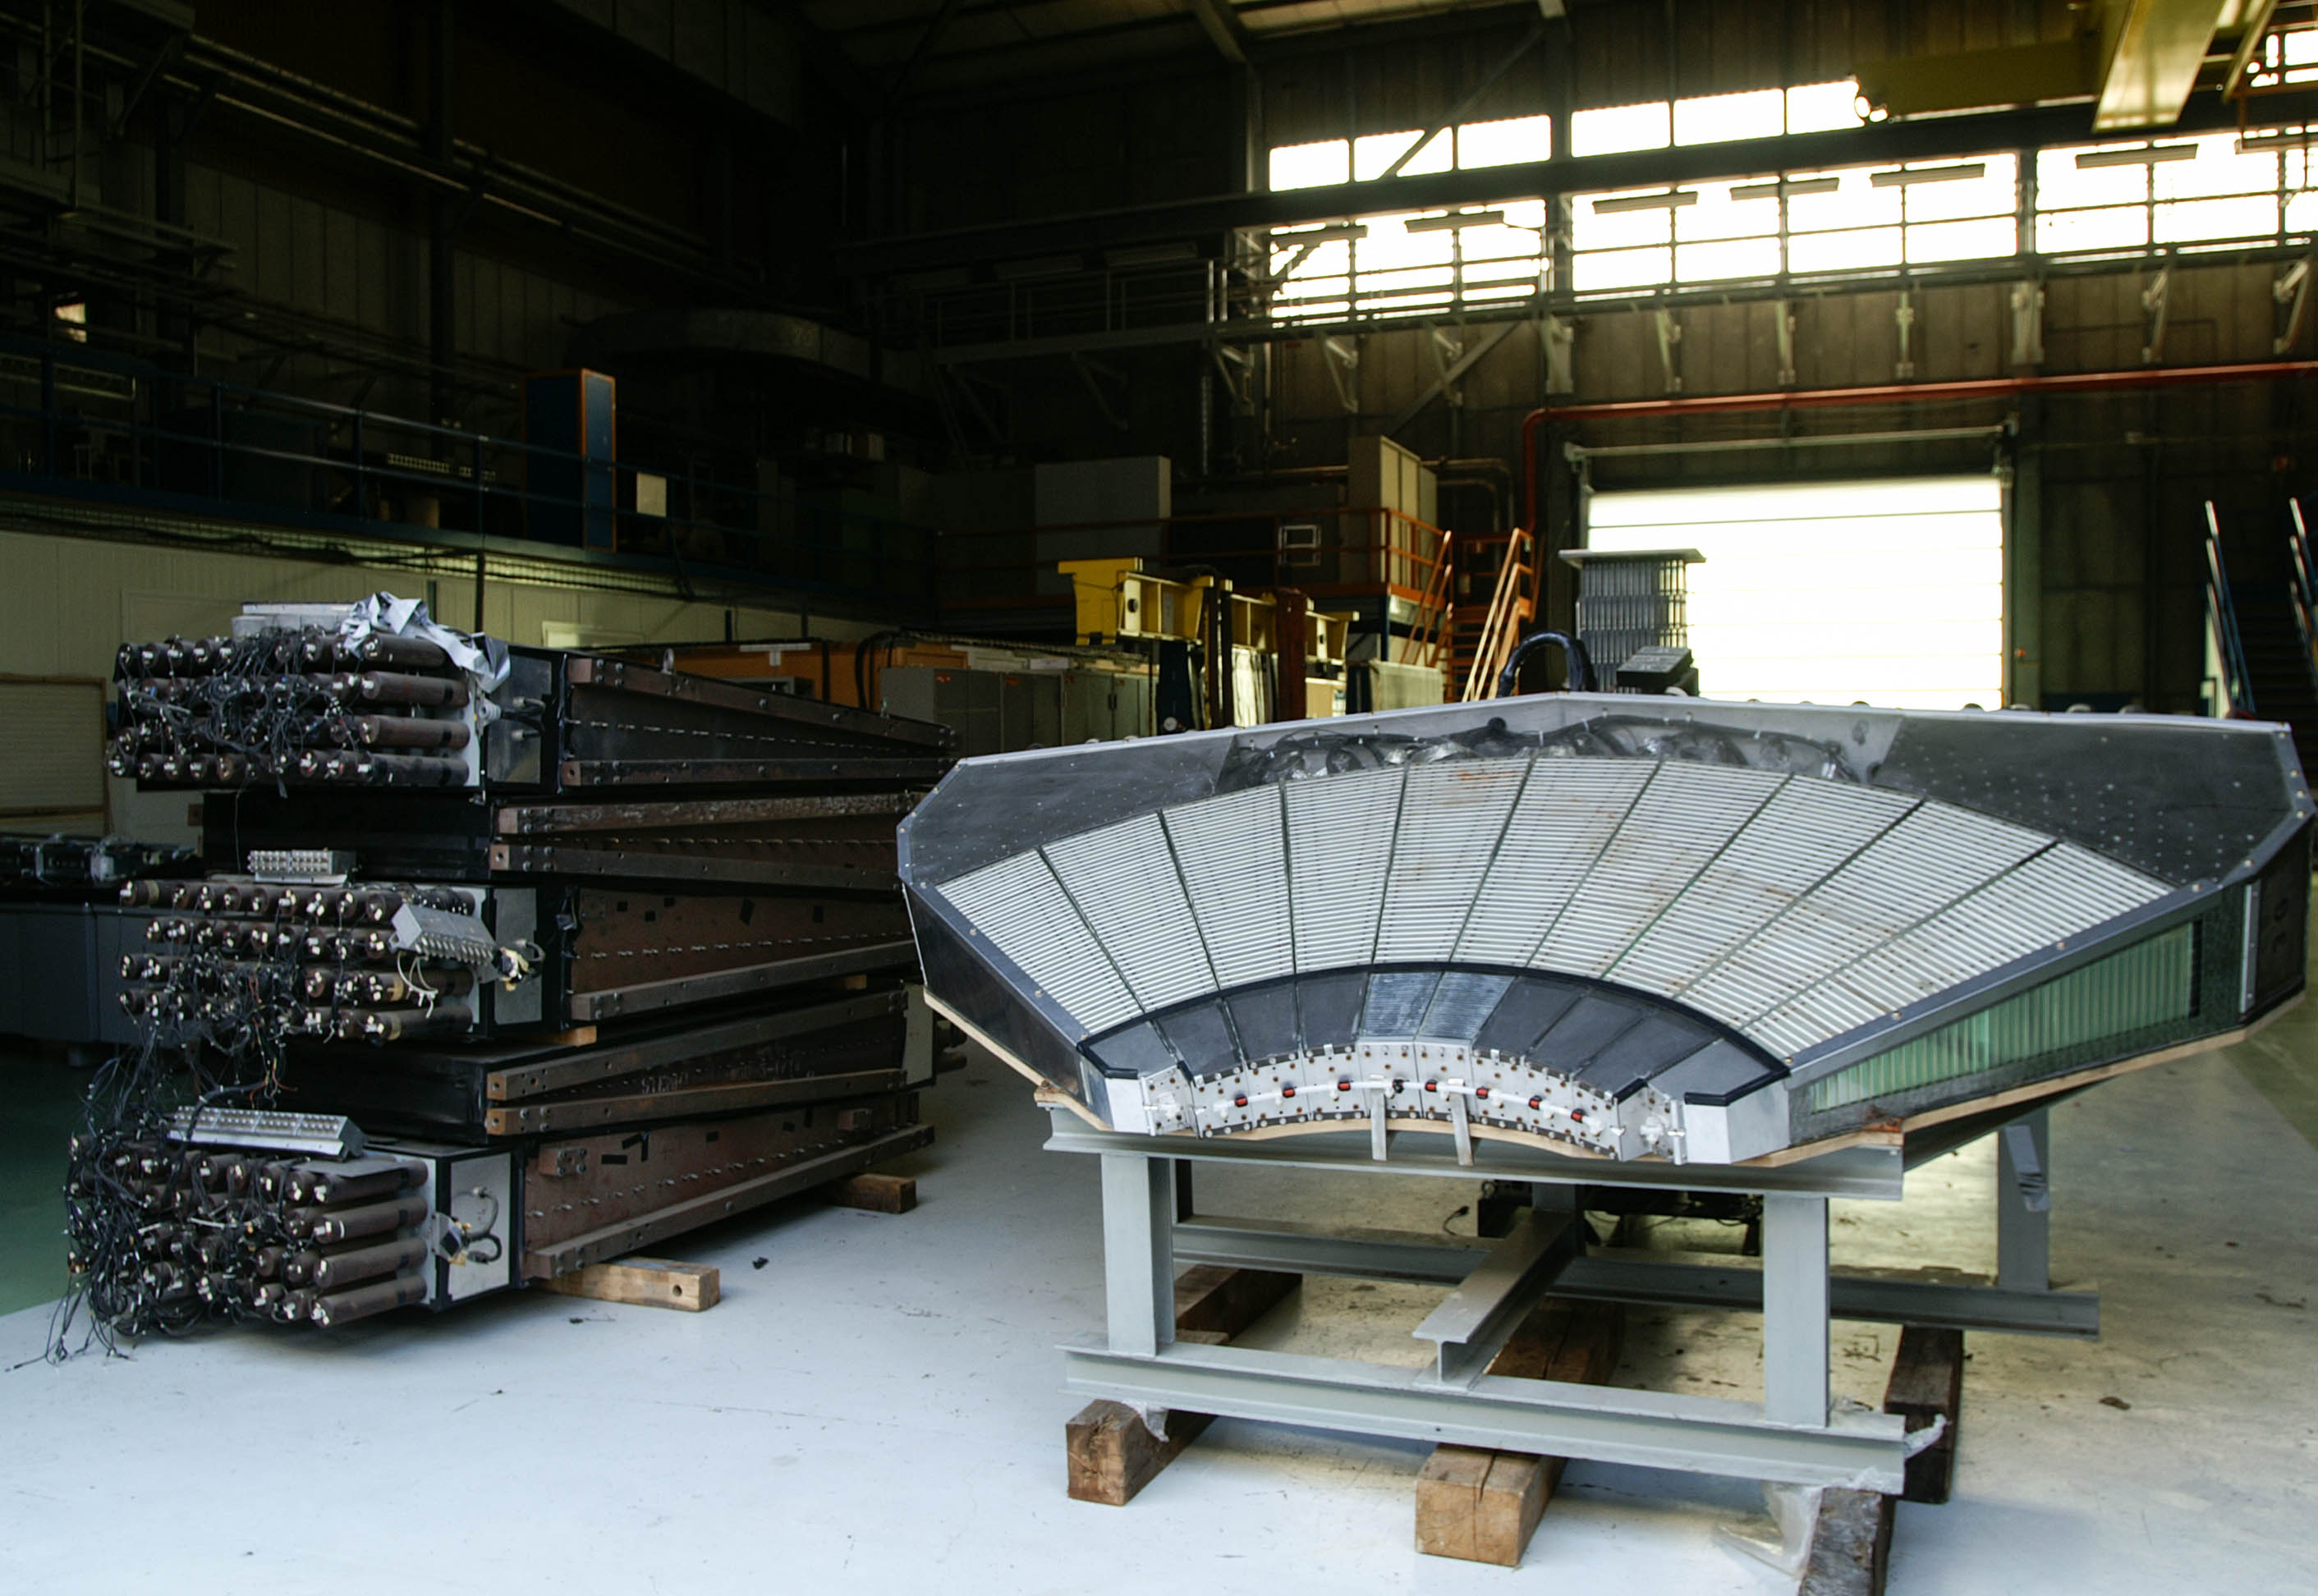
\includegraphics[width=\linewidth]{Images/Image1-Tilecal.jpg}
				\caption{Überreste eines Kalorimetermodules des UA2 Detektors (rechts) \cite{CERN-EX-8710495}}
	  			\label{fig:sad}
			\end{figure}
	\end{columns}
\end{frame}

\begin{frame}{Suche nach den W-Bosonen}
			\begin{itemize}
				\setlength\itemsep{0.5em}
				\item Suche nach $\text{W}^{\pm} \rightarrow \text{e}^{\pm} + \overset{(-)}{\nu_e}$ an UA1 und UA2
				\item Suche nach $\text{W}^{\pm} \rightarrow \mu^{\pm} + \overset{(-)}{\nu_\mu}$ an UA1
				\item Signatur von $\text{W} \rightarrow \text{e} \nu_\text{e}$:\\
				$\rightarrow$ Isoliertes Elektron mit hohem transversalen Impuls \\
				$\rightarrow$ Hoher fehlender transversaler Impuls durch Neutrino
				\item Fehlender transversaler Impuls:
				\begin{align*}
					\vec{p}_\text{T}^\text{miss} = - \sum_{\text{cells}} \vec{p}_\text{T}
				\end{align*}
				wobei über alle transversalen Impulsanteile in den Kalorimetern summiert wird
				\item Im idealen Detektor gilt: $\vec{p}_\text{T}^\text{miss} = \vec{p}_{\nu, \text{T}}$
			\end{itemize}

\end{frame}

\begin{frame}[plain]{Suche nach den W-Bosonen}
		\vspace*{-40px}
	\begin{columns}
		\column{0.4\textwidth}
			\begin{itemize}
				\setlength\itemsep{0.5em}
				\item Aufgetragen: Häufigkeit des Auftreten der fehlenden transversalen Impulse
				\item Bei kleinen Energien: Nicht signifikante fehlende transversale Impulse aufgrund von Kalorimeterauflösung
				\item In schwarz: Events, bei denen zusätzlich ein isoliertes Elektron mit hohem transversalen Impuls gefunden wurde
			\end{itemize}
		\column{0.6\textwidth}
			\begin{figure}
	  			\centering
				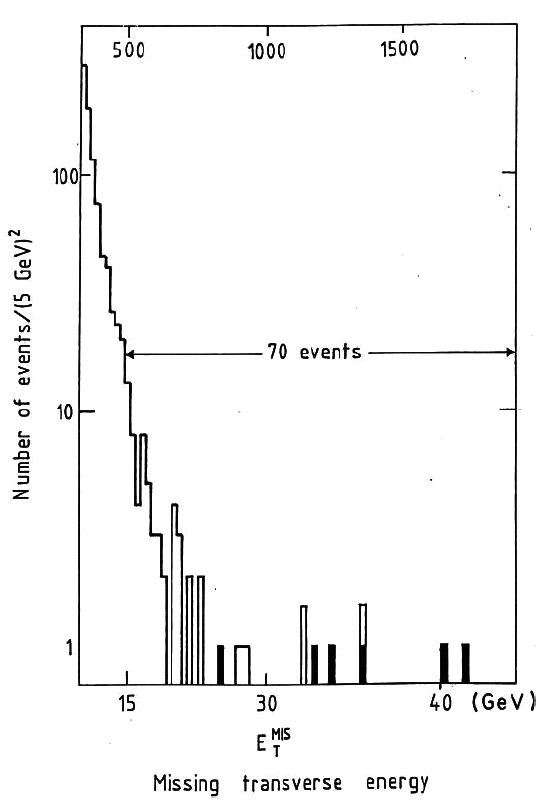
\includegraphics[width=0.65\textheight]{Images/Screenshot_2018-12-04_18-09-05.png}
				\caption{Ergebnisse von UA1, Daten aus dem Jahr 1982 \cite{doi:10.1142/9789814644150_0006}}
	  			\label{fig:sad}
			\end{figure}
	\end{columns}
\end{frame}

\begin{frame}[plain]{Suche nach den W-Bosonen}
		\vspace*{-40px}
	\begin{columns}
		\column{0.6\textwidth}
			\begin{figure}
	  			\centering
				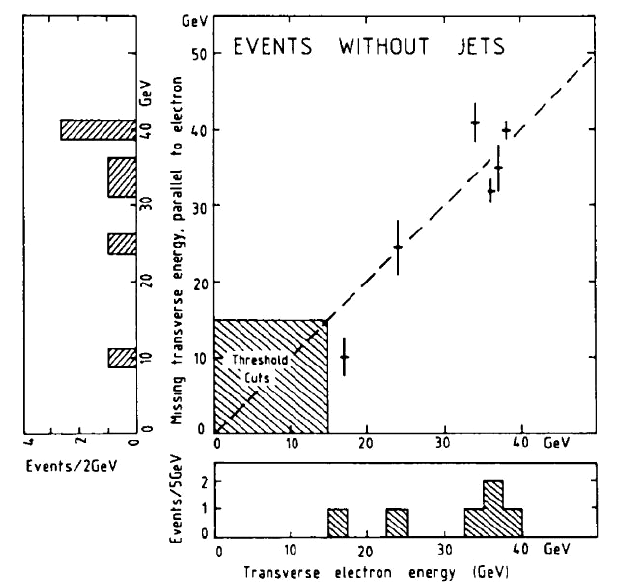
\includegraphics[width=0.95\textheight]{Images/Screenshot_2018-12-04_18-22-25.png}
				\caption{Ergebnisse von UA1, Daten aus dem Jahr 1982 \cite{doi:10.1142/9789814644150_0006}}
	  			\label{fig:sad}
			\end{figure}
		\column{0.35\textwidth}
				Transversaler Impuls der Elektronen und fehlender transversaler Impuls liegen "back to back" \\
				$\rightarrow$ Gesuchte Signatur!
	\end{columns}
\end{frame}

\begin{frame}{Suche nach den W-Bosonen}
	\begin{columns}
		\column{0.5\textwidth}
				\begin{itemize}
					\setlength\itemsep{0.5em}
					\vspace*{-20px}
					\item \textbf{20. Januar 1983} Ergebnis von UA1 wird in Seminar vorgestellt
					\item \textbf{21. Januar 1983} UA2 präsentiert sechs weitere Kandidaten
					\item \textbf{25. Januar 1983} Pressekonferenz mit der Nachricht, dass das W-Boson entdeckt wurde
					\item[$\rightarrow$] Im Bild von links nach rechts: Carlo Rubbia, Simon van der Meer, Herwig Schopper (Director General), Erwin Gabathuler (Research Director), Pierre Darriulat
				\end{itemize}
		\column{0.5\textwidth}
			\begin{figure}
	  			\centering
				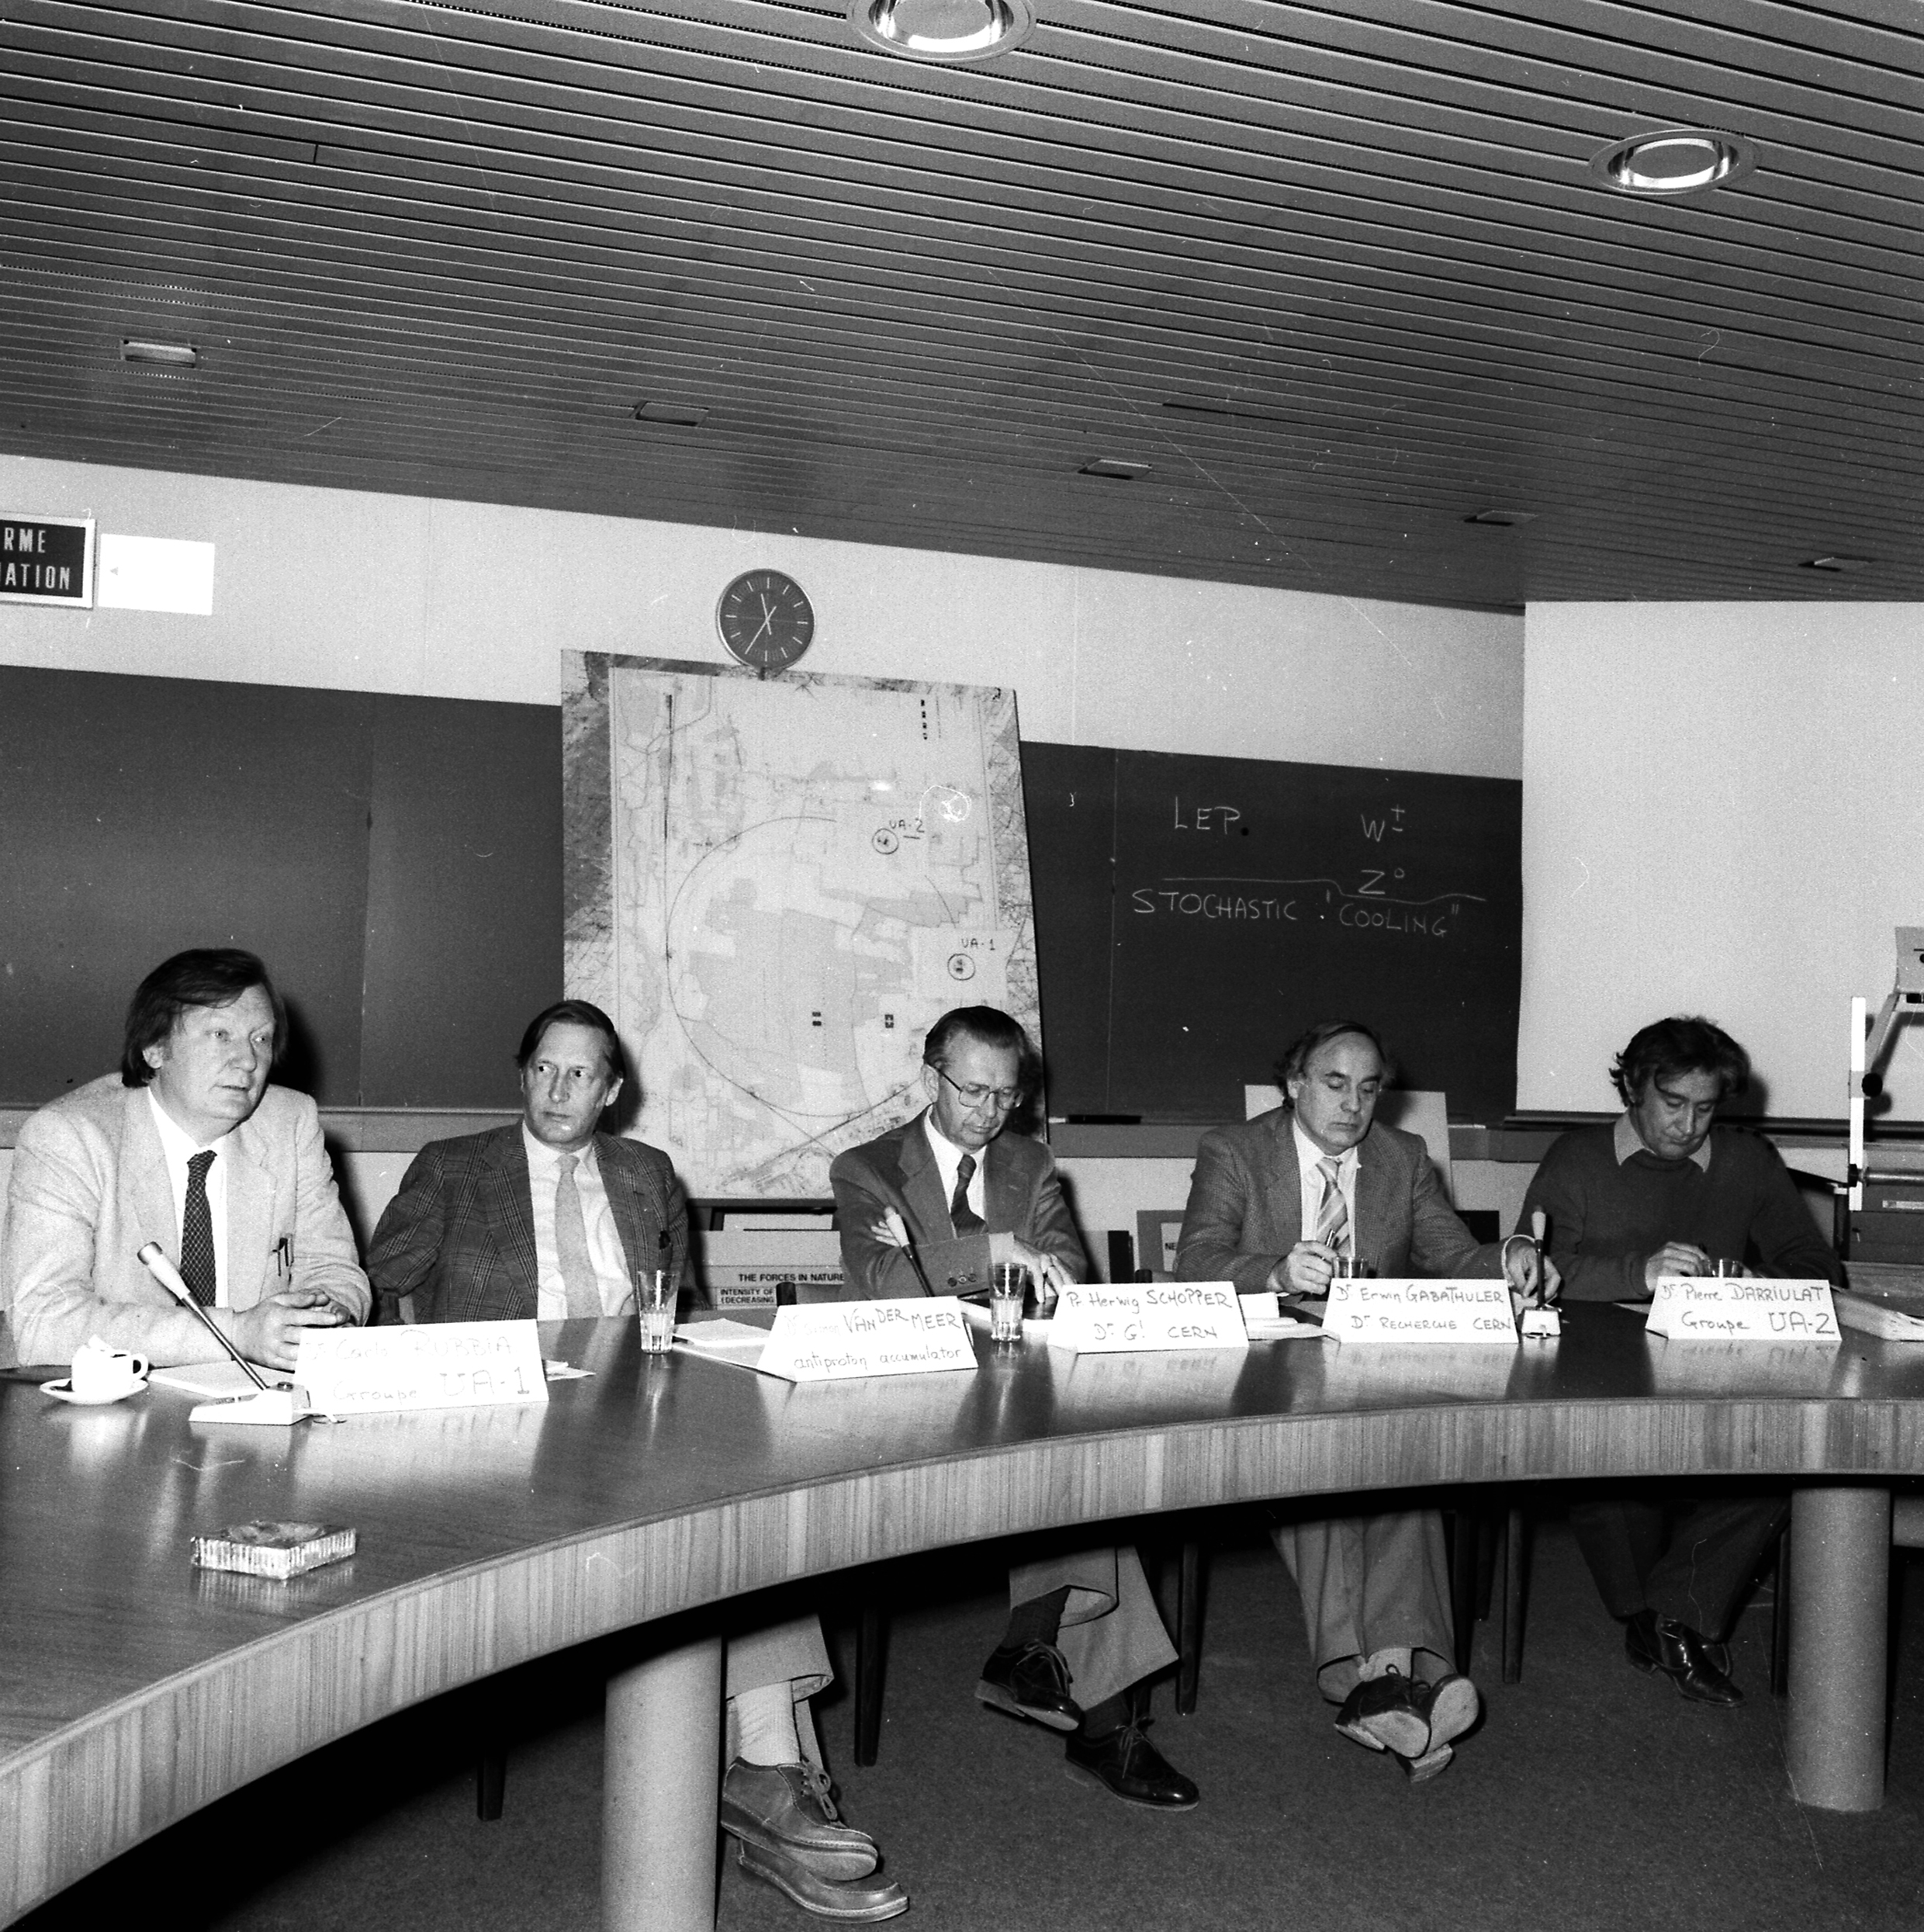
\includegraphics[width=0.85\linewidth]{Images/8301243}
				\caption{Pressekonferenz am 25. Januar 1983 \cite{CERN-HI-8301243}}
	  			\label{fig:sad}
			\end{figure}
	\end{columns}
\end{frame}

\begin{frame}{Suche nach dem Z-Boson}
			\begin{itemize}
				\setlength\itemsep{0.5em}
				\item Laut Theorie: Z-Boson Ereignisse treten etwa zehn mal seltener als W-Boson Ereignisse auf
				\item[$\rightarrow$] Längere Messzeit und Verbesserung der Luminosität
				\item Einschränkung der relevanten Events bei UA1:
				\item[1.] Zwei Kalorimetereinträge, die mit Elektronen kompatibel sind und ein $E_\text{T} > \SI{25}{\giga\electronvolt}$ besitzen
				\item[2.] Isolierte Spur, die auf einen der beiden Cluster zeigt
				\item[3.] Isolierte Spur, die auf zweiten Cluster zeigt
				\item[$\rightarrow$] 4 Events mit dieser Signatur gefunden, kompatibel mit einer eindeutigen invarianten Masse
			\end{itemize}
\end{frame}


\begin{frame}{Suche nach dem Z-Boson}
			\begin{figure}
	  			\centering
				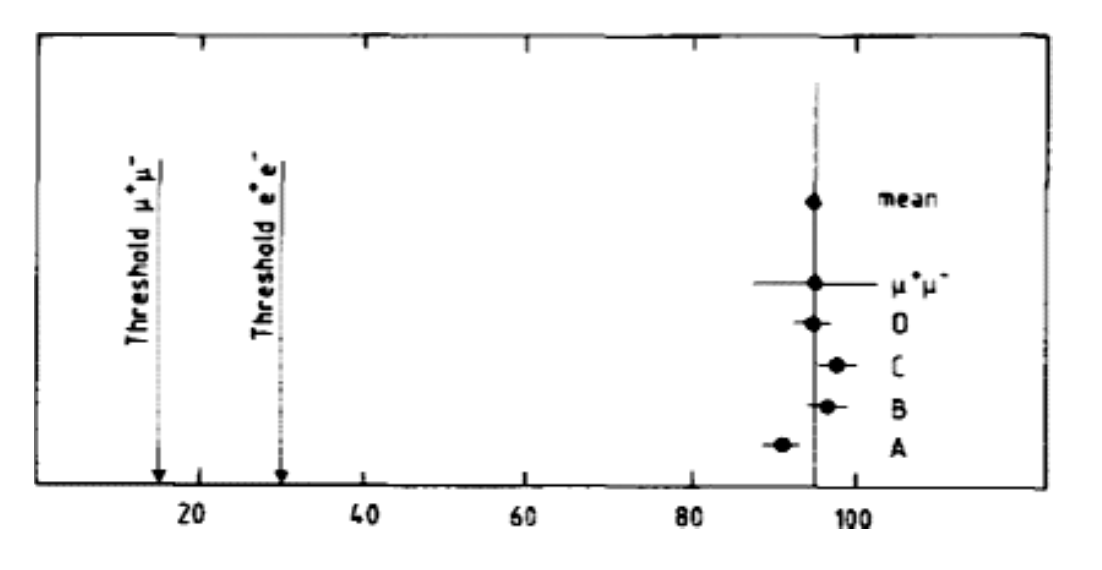
\includegraphics[width=0.85\linewidth]{Images/Screenshot_2018-12-05_15-29-02.png}
				\caption{Invariante Massen der Z-Boson-Ereignisse, die von UA1 beobachtet wurden. \cite{doi:10.1142/9789814644150_0006} Zusätzlich konnte ein Event mit der Signatur $\text{Z} \rightarrow \mu^+ \mu^-$ beobachtet werden.}
	  			\label{fig:sad}
			\end{figure}
\end{frame}

\begin{frame}{Suche nach dem Z-Boson}
	\begin{columns}
		\column{0.5\textwidth}
				\begin{itemize}
					\setlength\itemsep{0.5em}
					\vspace*{-20px}
					\item Wert für $M_\text{Z}$ von UA1:
					\begin{align*}
						M_\text{Z} = \left( \num{95.2} \pm \num{2.5} \pm \num{3.0} \right) \si{\giga\electronvolt}
					\end{align*}
					\item UA2 hat drei Kandidaten für Z-Bosonen gefunden, Wert für $M_\text{Z}$:
					\begin{align*}
						M_\text{Z} = \left( \num{91.9} \pm \num{1.3} \pm \num{1.4} \right) \si{\giga\electronvolt}
					\end{align*}
					\item Zum Vergleich: Der aktuelle Wert \cite{Patrignani:2016xqp}:
					\begin{align*}
						M_\text{Z} = \SI{91.1876+- 0.0021}{\giga\electronvolt}
					\end{align*}
					\item \textbf{1. Juni 1983}: Bekanntgabe, dass das Z-Boson gefunden wurde
				\end{itemize}
		\column{0.5\textwidth}
			\begin{figure}
	  			\centering
				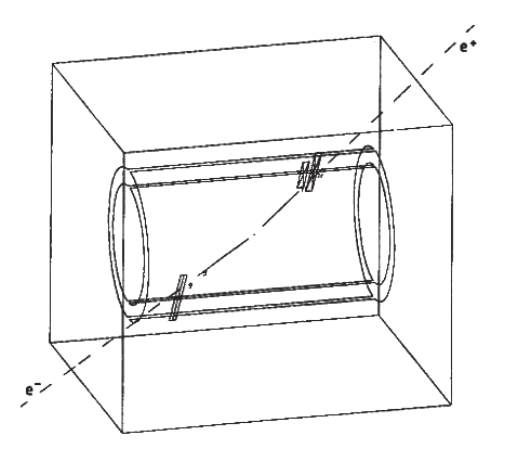
\includegraphics[width=0.85\linewidth]{Images/Screenshot_2018-12-05_15-33-31}
				\caption{Einzelnes UA1 Event der Signatur $\text{Z} \rightarrow \text{e}^+ \text{e}^-$, nachdem der Hintergrund entfernt wurde \cite{doi:10.1142/9789814644150_0006}}
	  			\label{fig:sad}
			\end{figure}
	\end{columns}
\end{frame}

\section{Die Zeit nach der Entdeckung}


\begin{frame}{Nobelpreise}
	\begin{columns}
		\column{0.5\textwidth}
				\begin{itemize}
					\setlength\itemsep{0.5em}
					\vspace*{-20px}
					\item \textbf{17. Oktober 1984} Der Nobelpreis in Physik wird an Carlo Rubbia und Simon Van der Meer vergeben: \\
					\emph{"For their decisive contributions to the large project, which led to the discovery of the field particles W and Z, communicators of weak interaction."}
				\end{itemize}
		\column{0.5\textwidth}
			\begin{figure}
	  			\centering
				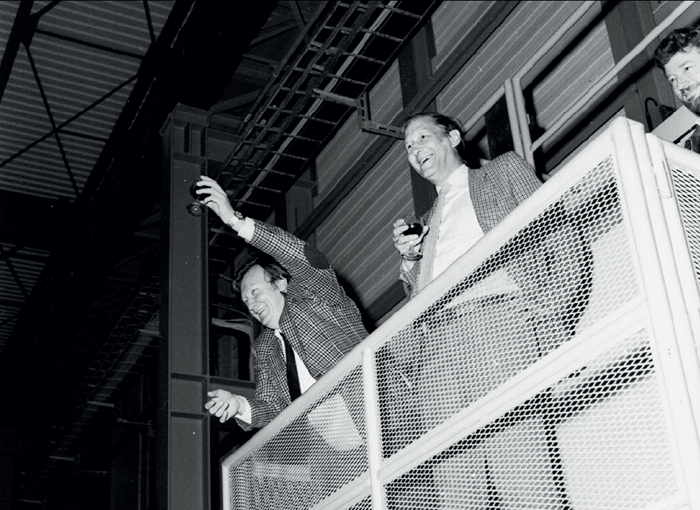
\includegraphics[width=\linewidth]{Images/CCint5_08_14}
				\caption{Carlo Rubbia und Simon van der Meer feiern den Erhalt des Nobelpreises am CERN \cite{CERN-PHOTO-8410523}}
	  			\label{fig:sad}
			\end{figure}
	\end{columns}
\end{frame}

\begin{frame}{Präsisionsmessungen}
	\begin{columns}
		\column{0.5\textwidth}
				\begin{itemize}
					\setlength\itemsep{0.5em}
					\vspace*{-20px}
					\item Präzisionsmessungen von $m_\text{W}$ und $m_\text{Z}$
					\item[$\rightarrow$] Am Large-Electron-Positron Collider (LEP), Betrieb von 1989 bis 2000
					\item[$\rightarrow$] Am Tevatron, Betrieb 1983 bis 2011
				\end{itemize}
		\column{0.5\textwidth}
			\begin{figure}
	  			\centering
				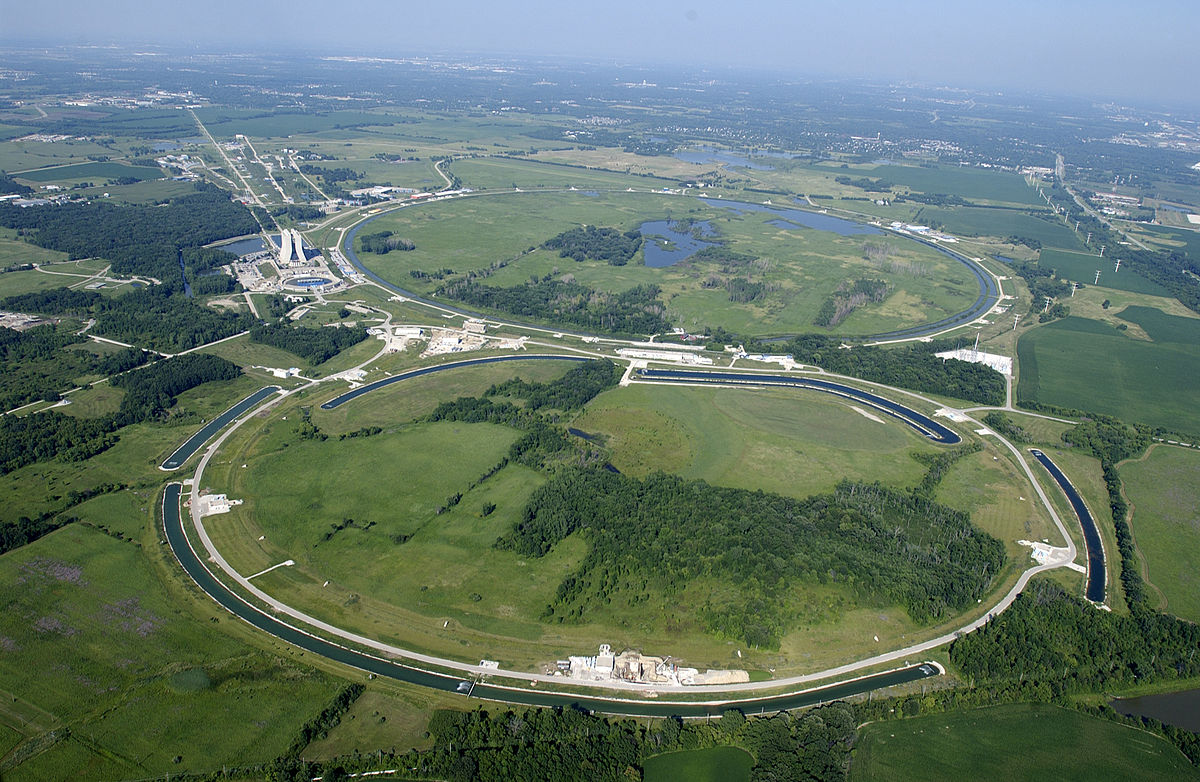
\includegraphics[width=\linewidth]{Images/1200px-Fermilab.jpg}
				\caption{Fermilab, Tevatron im Hintergrund \cite{wiki:tevatron}}
	  			\label{fig:sad}
			\end{figure}
	\end{columns}
\end{frame}

\begin{frame}{Präsisionsmessungen}
		\begin{figure}
	  		\centering
			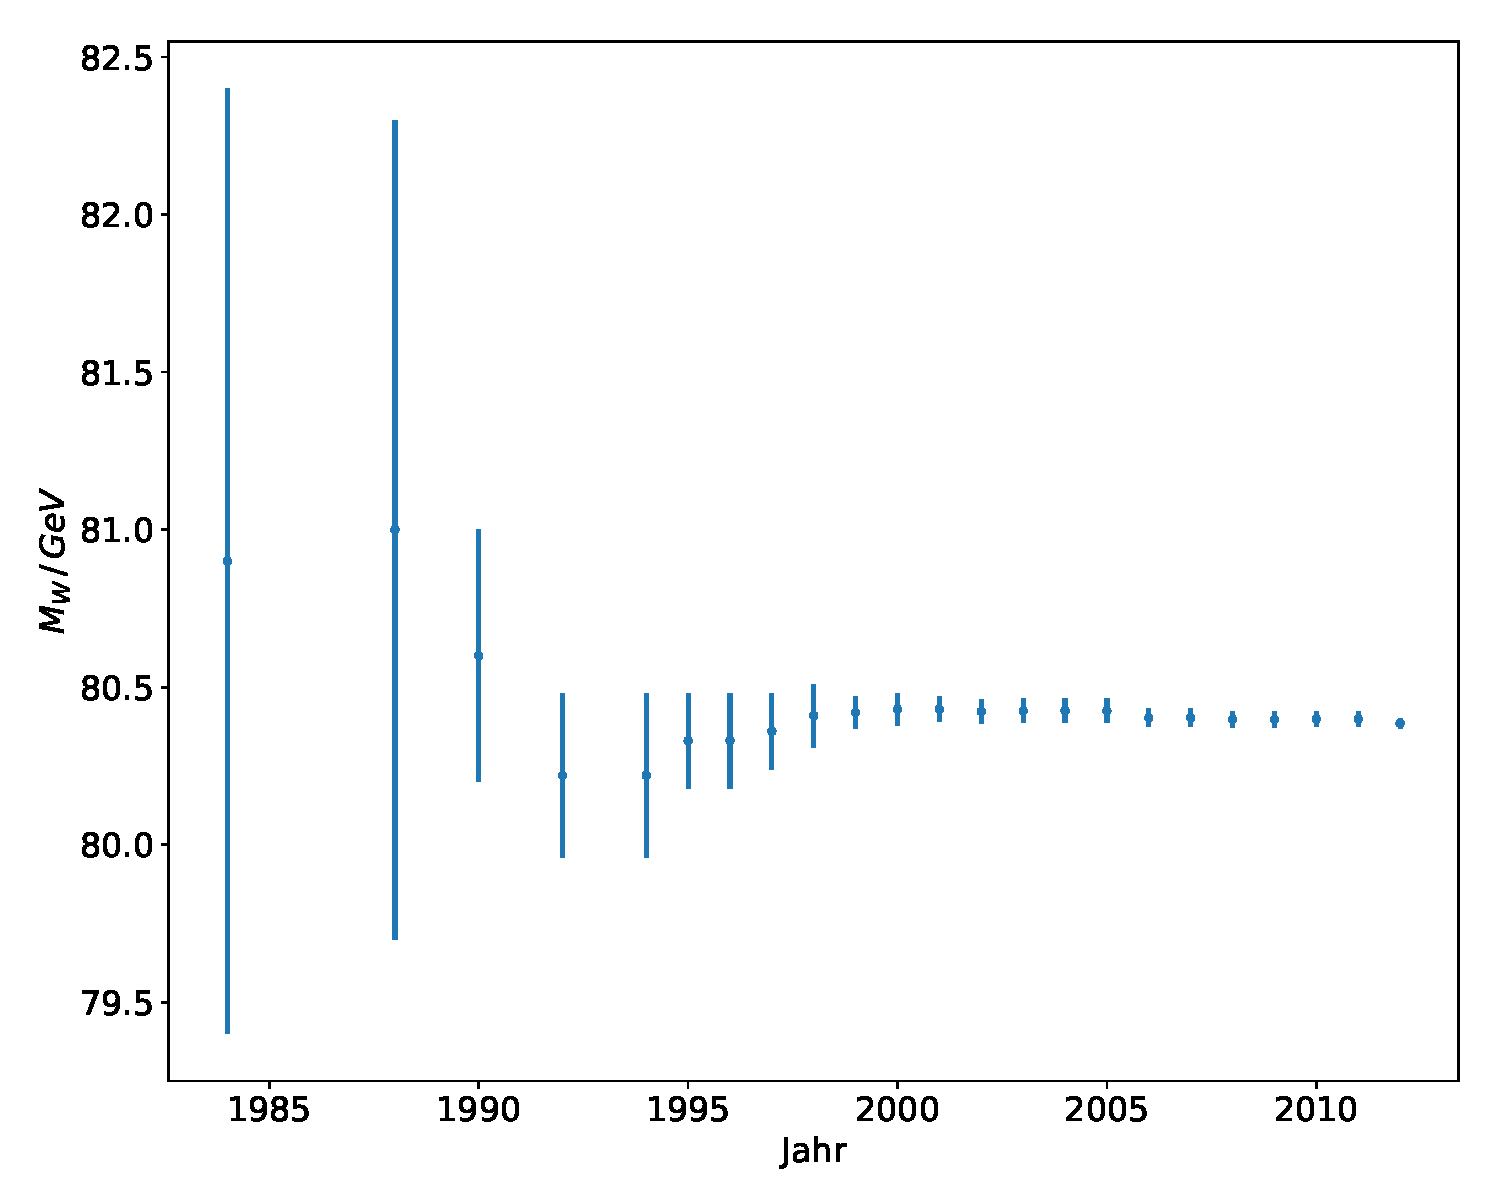
\includegraphics[width=0.9\textheight]{ressources/mw.pdf}
			\caption{Daten und Fehler für die Masse des W-Bosons für die verschiedenen Jahre aus dem PDG. Quelle: \url{http://pdg.lbl.gov/rpp-archive/}.}
	  		\label{fig:sad}
		\end{figure}
\end{frame}

\begin{frame}{Präsisionsmessungen}
		\begin{figure}
	  		\centering
			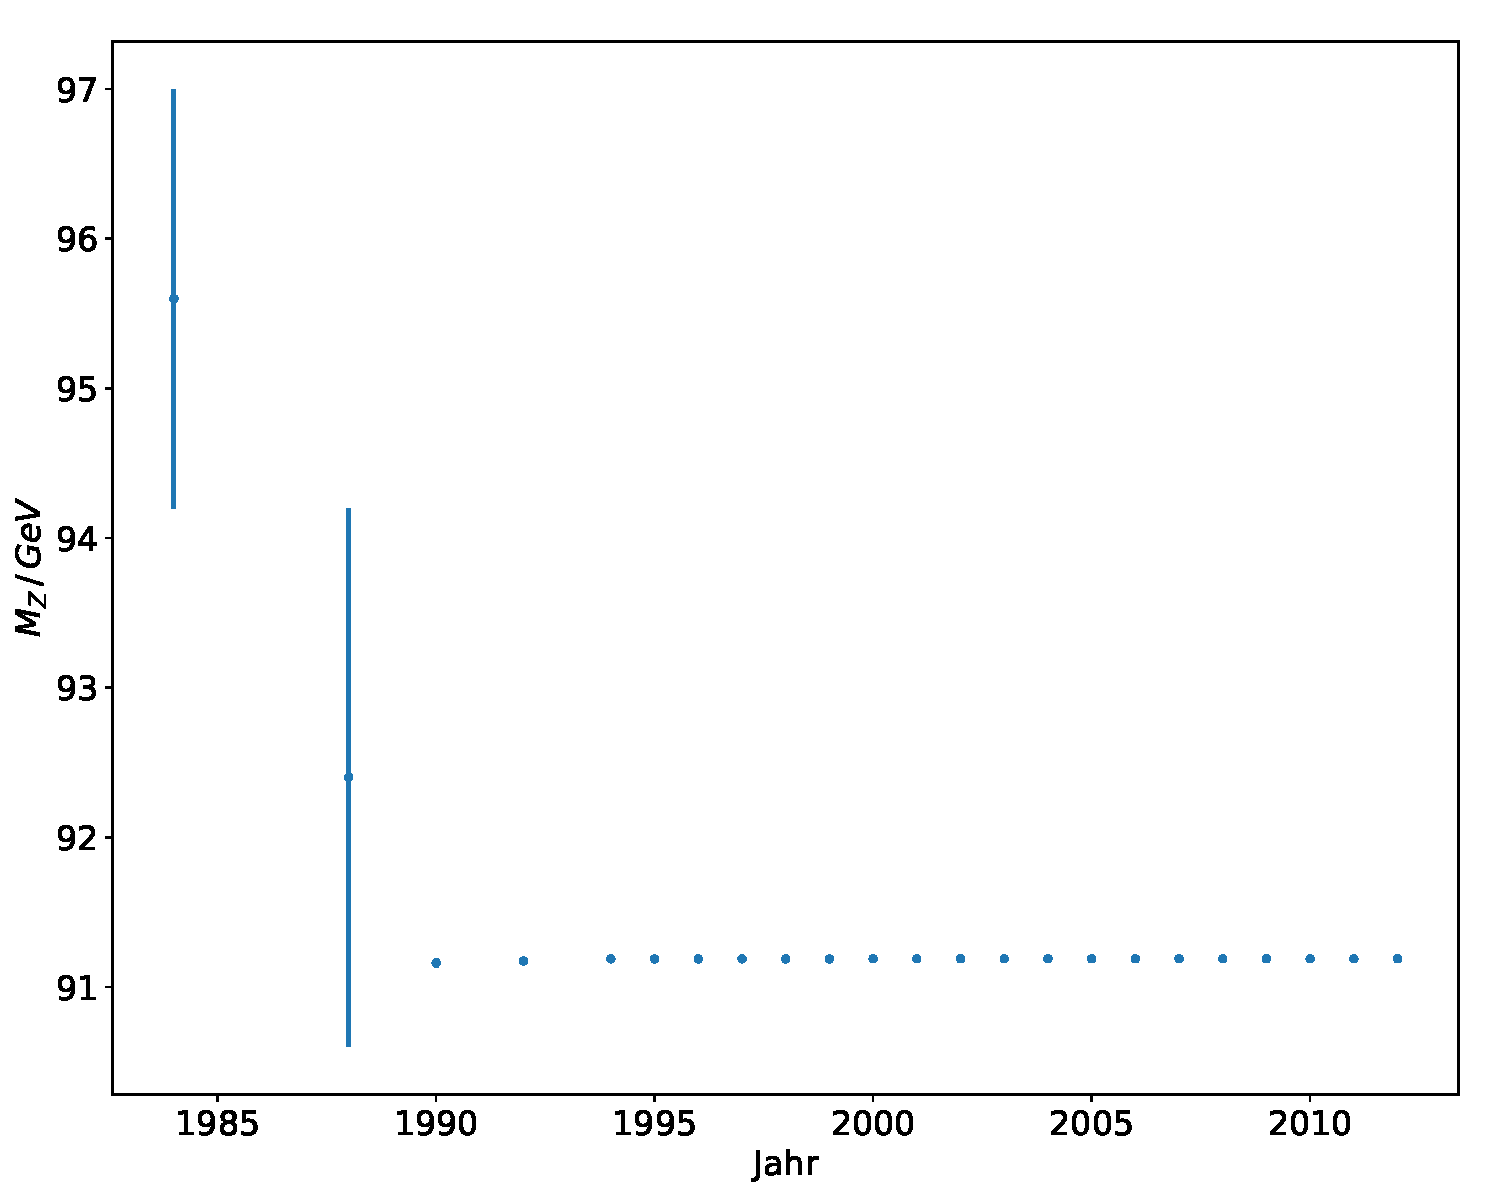
\includegraphics[width=0.9\textheight]{ressources/mz.pdf}
			\caption{Daten und Fehler für die Masse des Z-Bosons für die verschiedenen Jahre aus dem PDG. Quelle: \url{http://pdg.lbl.gov/rpp-archive/}.}
	  		\label{fig:sad}
		\end{figure}
\end{frame}

\begin{frame}{Zusammenfasung}
	\begin{chronology}[3]{1967}{1985}{\textwidth}		
		\event{1968}{Theorie der elektroschwachen Wechselwirkung}
		\event{1973}{Beobachtung der neutralen Ströme (Gargamelle)}
		\event{1978}{Umbau des SPS zu p$\overline{\text{p}}$-Collider}
		\event{1981}{Entdeckung W und Z (UA1 und UA2)}
		\event{1984}{Nobelpreis für Rubbia und Van der Meer}
	\end{chronology}
\end{frame}


%------------------------------------------------

\begin{frame}[focus]
	Vielen Dank für die Aufmerksamkeit!
\end{frame}

%----------------------------------------------------------------------------------------
%	 CLOSING/SUPPLEMENTARY SLIDES
%----------------------------------------------------------------------------------------

\appendix

\setbeamertemplate{bibliography item}[text]


\begin{frame}[allowframebreaks]{References}
	\bibliography{example.bib}
	\bibliographystyle{unsrt}
\end{frame}

%------------------------------------------------

\begin{frame}{Vorhersage der W- und Z-Boson Massen}
			Aus der elektroschwachen Theorie folgt \cite{vorhersage}
			\begin{align*}
				\frac{\sigma_\text{NC}}{\sigma_\text{CC}} = \frac{1}{2} - \sin^2{\left( \Theta_\text{W}\right)} + \frac{20}{27} \sin^4{\left( \Theta_\text{W}\right)}
			\end{align*}
			sowie
			\begin{align*}
				M_\text{W}^2 &= \frac{e^2 \sqrt{2}}{8 \text{G}_\text{F} \sin^2{\left( \Theta_\text{W}\right)} }\\
				M_\text{Z} &= \frac{M_\text{W}}{\cos{\left( \Theta_\text{W}  \right)}}.
			\end{align*}
			Hieraus lassen sich aus den experimentellen Daten von Gargamelle die Massen des W-Bosons und Z-Bosons vorhersagen zu
			\cite{doi:10.1142/9789814644150_0006}:
			\begin{align*}
				M_\text{W} &\approx \left(60-80\right)\si{\giga\electronvolt}\\
				M_\text{Z} &\approx \left(75-92\right)\si{\giga\electronvolt}
			\end{align*}
\end{frame}

\begin{frame}{Messung der W-Boson Masse von UA1}
				\begin{itemize}
					\setlength\itemsep{0.5em}
					\vspace*{-20px}
					\item Beobachtung von $\text{W} \rightarrow \text{e} \nu$
					\item Invariante Masse lässt sich aufgrund des nicht detektierten Neutrinos nicht vollständig bestimmen
					\item[$\rightarrow$] $z$-Komponente des Impulses ist unbekannt
				\end{itemize}
				Betrachte transversale Masse $M_\text{T}$, definiert über
				\begin{align*}
					M_\text{T}^2 = \left( E_{\text{T}, 1} + E_{\text{T}, 2} \right) - \left( \vec{p_{\text{T}, 1}} + \vec{p_{\text{T}, 2}} \right)
				\end{align*}
				mit $E_\text{T} \approx |\vec{p_{\text{T}, 1}}|$. Es ergibt sich
				\begin{align*}
					M_\text{T}^2 = 2 E_{\text{T}, 1} E_{\text{T}, 2} \left( 1 - \cos{\Theta} \right)
				\end{align*}
				mit dem Winkel $\Theta$ zwischen den beiden Zerfallsprodukten.
\end{frame}


\begin{frame}{Messung der W-Boson Masse von UA1}
	\begin{columns}
		\column{0.4\textwidth}
				\begin{itemize}
					\setlength\itemsep{0.5em}
					\vspace*{-20px}
					\item Transversale Masse $M_\text{T}$ ist sensitiv auf $M_\text{W}$
					\item[$\rightarrow$] Auftreten der "Jacobi-Kante" bei $M_\text{W}$, wenn $M_\text{T}$ gegen die Ereignisrate aufgetragen wird
					\item[$\rightarrow$] Grund: $M_\text{T} \leq M_\text{W}$
					\item[$\rightarrow$] Kante verschmiert aufgrund von endlicher Zerfallsbreite sowie Impuls in $z$-Richtung
					\item Bestimmung von $M_\text{W}$ zu \cite{doi:10.1142/9789814644150_0006}
					\begin{align*}
						M_\text{W} = \left( \num{80.2} \pm \num{0.8} \pm \num{1.3} \right)\si{\giga\electronvolt}
					\end{align*}
				\end{itemize}
		\column{0.6\textwidth}
			\begin{figure}
	  			\centering
				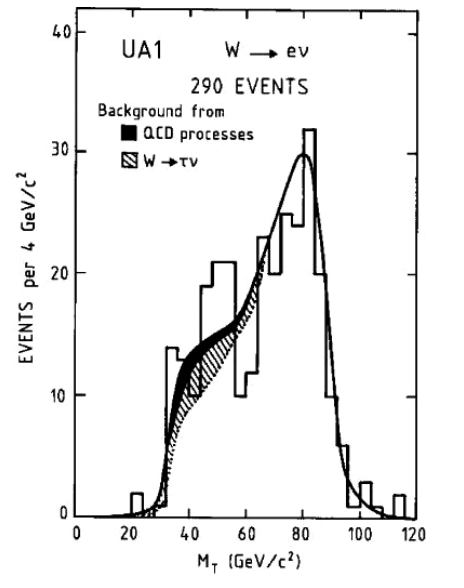
\includegraphics[width=0.7\linewidth]{Images/Screenshot_2018-12-05_16-22-51.png}
				\caption{Transversale Masse $M_\text{T}$ in der Signatur $\text{W} \rightarrow \text{e} \nu$, gemessen von UA1 \cite{doi:10.1142/9789814644150_0006}}
	  			\label{fig:sad}
			\end{figure}
	\end{columns}
\end{frame}


%----------------------------------------------------------------------------------------

\end{document}
